%You can leave alone everything before Line 79.
\documentclass{article}
\usepackage{url,amsfonts, amsmath, amssymb, amsthm,color, enumerate, verbatim}
% Page layout
\setlength{\textheight}{8.75in}
\setlength{\columnsep}{2.0pc}
\setlength{\textwidth}{6.5in}
\setlength{\topmargin}{0in}
\setlength{\headheight}{0.0in}
\setlength{\headsep}{0.0in}
\setlength{\oddsidemargin}{0in}
\setlength{\evensidemargin}{0in}
\setlength{\parindent}{1pc}
\newcommand{\shortbar}{\begin{center}\rule{5ex}{0.1pt}\end{center}}
%\renewcommand{\baselinestretch}{1.1}
% Macros for course info
\newcommand{\courseNumber}{ME 552}
\newcommand{\courseTitle}{Mechatronics}
\newcommand{\semester}{Fall 2012}
\newcommand{\xxx}[1]{\textcolor{red}{#1}}
% Theorem-like structures are numbered within SECTION units
\theoremstyle{plain}
\newtheorem{theorem}{Theorem}[section]
\newtheorem{lemma}[theorem]{Lemma}
\newtheorem{corollary}[theorem]{Corollary}
\newtheorem{proposition}[theorem]{Proposition}
\newtheorem{statement}[theorem]{Statement}
\newtheorem{conjecture}[theorem]{Conjecture}
\newtheorem{fact}{Fact}
%definition style
\theoremstyle{definition}
\newtheorem{definition}[theorem]{Definition}
\newtheorem{example}{Example}
\newtheorem{problem}[theorem]{Problem}
\newtheorem{exercise}{Exercise}
\newtheorem{algorithm}{Algorithm}
%remark style
\theoremstyle{remark}
\newtheorem{remark}[theorem]{Remark}
\newtheorem{reduction}[theorem]{Reduction}
%\newtheorem{question}[theorem]{Question}
\newtheorem{question}{Question}
%\newtheorem{claim}[theorem]{Claim}
%
% Proof-making commands and environments
\newcommand{\beginproof}{\medskip\noindent{\bf Proof.~}}
\newcommand{\beginproofof}[1]{\medskip\noindent{\bf Proof of #1.~}}
\newcommand{\finishproof}{\hspace{0.2ex}\rule{1ex}{1ex}}
\def\therefore{\boldsymbol{\text{ }
\leavevmode
\lower0.4ex\hbox{$\cdot$}
\kern-.5em\raise0.7ex\hbox{$\cdot$}
\kern-0.55em\lower0.4ex\hbox{$\cdot$}
\thinspace\text{ }}}

\newenvironment{solution}[1]{\medskip\noindent{\bf Problem #1.~}}{\shortbar}

%====header======
\newcommand{\solutions}[4]{
%\renewcommand{\thetheorem}{{#2}.\arabic{theorem}}
\vspace{-2ex}
\begin{center}
{\small  \courseNumber, \courseTitle
\hfill {\Large \bf {#1} }\\
\semester, University of Michigan, Ann Arbor \hfill
{\em Date: #3}}\\
\vspace{-1ex}
\hrulefill\\
\vspace{4ex}
{\LARGE Lab Assignment #2}\\
\vspace{2ex}
\end{center}
\begin{trivlist}
\item \textsc{Team members:\\} {#4}
\end{trivlist}
\noindent
\shortbar
\vspace{3ex}
}
% math macros
\newcommand{\defeq}{\stackrel{\textrm{def}}{=}}
\newcommand{\Prob}{\textrm{Prob}}
\newcommand{\Lagr}{\mathcal{L}}
%==
\usepackage{graphicx}
\usepackage{xfrac}
\usepackage{amsmath}
\providecommand{\e}[1]{\ensuremath{\times 10^{#1}}}
\begin{document}
%%%%%%%%%%%%%%%%%%%%%%%%%%%%%%%%%%%%%%%%%%%%%%%%%
%\solutions{Your name}{Problem Set Number}{Date of preparation}{Collaborators}{Prover}{Verifiers}
\solutions{}{4: Inverted Pendulum}{\today}{Shiva Ghose, @gshiva\\ John Peterson, @jrpeters\\ Peter Turpel, @pturpel\\ Chan-Rong Lin, @pmelin}
%%%%%%%%%%%%%%%%%%%%%%%%%%%%%%%%%%%%%%%%%%%%%%%%%
%\renewcommand{\theproblem}{\arabic{problem}} 
%%%%%%%%%%%%%%%%%%%%%%%%%%%%%%%%%%%%%%%%%%%%%%%%%
%
% Begin the solution for each problem by
% \begin{solution}{Problem Number} and ends it with \end{solution}
%
% the solution for Problem 
\section*{Teamwork Participation Pledge :: Team 1}

I attest that I have made a fair and equitable contribution to this lab and submitted 
assignment. \\

My signature also indicates that I have followed the University of Michigan Honor Code, 
while working on this lab and assignment.\\

I accept my responsibility to look after all of the equipment assigned to me and my team, 
and that I have read and understood the X50 Lab Rules.\\

\begin{table}[h]
\begin{center}
    \begin{tabular}{|c|c|c|}
        \hline
        \textbf{Name} & \textbf{Email}     & \textbf{ \ \ \ \ \  \ \  \ \ \ \ \  \ \ Signature  \ \ \ \ \  \ \ \ \ \ \ \  \ \ } \\ \hline
        	~& ~& ~\\
	~& ~& ~\\
	Shiva Ghose   & gshiva@umich.edu   & ~                  \\
	~& ~& ~\\
	~& ~& ~\\ \hline 
	~& ~& ~\\
	~& ~& ~\\
        John Peterson & jrpeters@umich.edu & ~                  \\ 
	~& ~& ~\\
	~& ~& ~\\ \hline 
	~& ~& ~\\
	~& ~& ~\\
        Peter Turpel   & pturpel@umich.edu & ~                  \\
	~& ~& ~\\
	~& ~& ~\\ \hline 
	~& ~& ~\\
	~& ~& ~\\
        Chan-Rong Lin   & pmelin@umich.edu & ~                  \\
	~& ~& ~\\
	~& ~& ~\\ \hline 
        \hline
    \end{tabular}
\end{center}
\end{table}

\newpage

\section{System Modeling}

\begin{figure}[htb]
\begin{center}
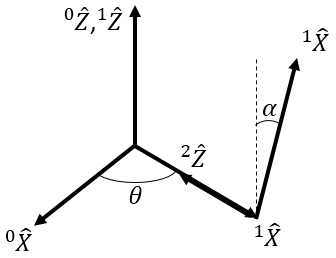
\includegraphics[width = 6cm]{coordinates.png}
\caption{The co-ordinate frames of the inverted pendulum system}
\label{q1_coords}
\end{center}
\end{figure}

\subsection*{a. Physical Model}
We model the physical system as a pair of rigid links, the horizontal arm and the pendulum mounted to the end of the arm, neglecting the presence of the encoder cable, using a lumped parameter model.

\subsection*{b. Assumptions}
We make the following assumptions while modeling the system:
\begin{itemize}
\item All of the links are rigid - this allows us to neglect work done by the internal constraining forces of the system as well as losses due to collisions and deformations. This assumption very nearly holds because system is built using stiff metals and bearings that are well fitted.

\item Air resistance is neglected - this is due to the small cross sectional areas and low velocities experienced by the system. Additionally this is neglected due to the difficulty in constructing an appropriate model for these losses.

\item The axis of rotation of the horizontal arm is perfectly level with the ground -  this assumption ensures that there will be no potential energy term associated with the arm.

\item The presence of the encoder cable connected to the arm is neglected - We found that the cable has a large impact on our system however its influence would be very difficult to model because it is not fixed to the arm and because the forces it introduces are highly non linear.   
\end{itemize}

Apart from the above list, the standard set of control systems assumptions are also made:
\begin{itemize}
\item The current driver acts instantaneously - the transients involved occur so quickly with respect to the system response time that we virtually have immediate response. Also, the motor, acting as a low pass filter, will reject the high frequency components of the driver.

\item The DAQ has instantaneous and correct response - we ignore the quantization and discretization errors of the DAQ and further assume that offset errors have been accounted for. This is valid because our control loop runs at 100 Hz while the DAQ can be sampled at 1000 Hz. Additionally we believe that the DAQ has been calibrated and static errors have been removed.
\end{itemize}


\subsection*{c. Mathematical Modeling}
\subsubsection*{Forwards Kinematics}
Let $^0F$ represent the fixed world coordinate frame, with $\bf{^0\hat{z}}$ aligned with the motor shaft and with $\bf{^0\hat{x}}$ pointing along the initial direction of the horizontal arm as seen in figure \ref{q1_coords} on page \pageref{q1_coords}.  Let the origin of $^0F$ be located to coincide with the motor axis and the axis of rotation of the pendulum.  Let $^1F$, representing the local frame of the horizontal arm, be attached to the horizontal arm, with $\bf{^1\hat{z}}$ aligned with the motor shaft and $\bf{^1\hat{x}}$ aligned with the motor arm pointed towards the pendulum.  Let $^2F$ be located such that its origin is along $\bf{^1\hat{x}}$ at a distance $l_1$, with $\bf{^2\hat{x}}$ pointing along the pendulum and $\bf{^2\hat{z}}$ along the $\bf{-^1\hat{x}}$ direction.  Where $l_1$ is the distance from the axis of rotation of the motor to the center of mass of the pendulum along the $\bf{^1\hat{x}}$ direction, shown in figure \ref{q2_5}.  Let $\theta$ denote the angle between $\bf{^0\hat{x}}$ and $\bf{^1\hat{x}}$ and let $\alpha$ denote the angle between $\bf{^1\hat{z}}$ and $\bf{^2\hat{x}}$ measured clockwise when viewed from $\bf{^1\hat{x}}$.  We assume that the motor and the horizontal arm are rigidly connected and can be treated as a single inertia for purposes of our energy calculations below.\\

Then:

$$ ^0F = R_{z}(\theta) T_{x}(l_{1}) R_{y}(-\sfrac{\pi}{2}) R_{z}(\alpha) \left(^2F\right) $$

Let $l_{2c}$ be the distance along $\bf{^2x}$ from the origin of $^2F$ to the center of mass of the pendulum, shown in figure \ref{q2_3}.  Then the location of the center of mass of the pendulum in the world coordinate system $\bf{^0P_{2c}}$ is given as:

$$ {\bf{^0P_{2c}}} = R_{z}(\theta) T_{x}(l_{1}) R_{y}(-\sfrac{\pi}{2}) R_{z}(\alpha) \left(\bf{^2P_{2c}}\right) = R_{z}(\theta) T_{x}(l_{1}) R_{y}(-\sfrac{\pi}{2}) R_{z}(\alpha) \left[l_{2c}, 0, 0\right]^T$$

\[
  {\bf{^0P_{2c}}} = \left[
  \begin{array}{c l}
	 -l_{2c} \sin(\theta) \sin(\alpha) + l_{1} \cos(\theta) \\
	l_{2c} \cos(\theta) \sin(\alpha) + l_1 \sin(\theta) \\
	l_{2c} \cos(\alpha) 
  \end{array} \right]
\]

From this position we can then determine the linear velocity of the center of mass of the pendulum in the world frame denoted $\bf{^0\dot{P}_{2c}}$.  Let $J$ denote the matrix of partial derivatives of $\bf{^0P_{2c}}$ with respect to $\theta$ and $\alpha$.  Then the $\bf{^0\dot{P}_{2c}}$ is given by:

$$ {\bf{^0\dot{P}_{2c}}} = J \left[ \begin{array}{c l} \dot{\theta} \\ \dot{\alpha} \end{array} \right] = \left[ \begin{array}{c c l} 
	-l_{2c} sin(\alpha) \cos(\theta) - l_{1} \sin(\theta)  &  -l_{2c} \sin(\theta) \cos(\alpha) \\
	-l_{2c} sin(\alpha) \sin(\theta) + l_1 \cos(\theta) & l_{2c} \cos(\theta) \cos(\alpha) \\
	0 & -l_{2c} \sin(\alpha) \\ \end{array} \right] \left[ \begin{array}{c l} \dot{\theta} \\ \dot{\alpha} \end{array} \right]$$

We can also determine the angular velocity of the pendulum about its center of mass in the pendulum fixed frame $^2F$  by the following:

$$ {\bf{\omega_{2}}}= \dot{\theta} ({\bf{^1\hat{z}}}) + \dot{\alpha}({\bf{^2\hat{z}}})  = \left( R_{y}(-\sfrac{\pi}{2}) R_{z}(\alpha)\right)^{-1} \left[ 0, 0, \dot{\theta} \right]^T + \dot{\alpha}({\bf{^2\hat{z}}})$$

$$  {\bf{^2\omega_{2}}}= \left[ \begin{array}{c l}   \dot{\theta} \cos(\alpha) \\ -\dot{\theta} \sin(\alpha) \\ \dot{\alpha} \end{array} \right]$$

Rather than concern ourselves with the forward kinematics of the horizontal arm, we assume that its only motion is a rotation about $\bf{^0\hat{z}}$ which allows us to simply apply the parallel axis theorem to obtain its moment of inertia about $\bf{^0\hat{z}}$.


\subsubsection*{System Energy}

Our system is composed of two rigid bodies, the horizontal arm and the pendulum.  Each has an energy denoted $E_1$ and $E_2$ respectively.  Using the forward kinematics derived above we can compute the kinetic and potential energies associated with each body as a function of $\theta$, $\alpha$, $\dot{\theta}$, and $\dot{\alpha}$.

$$ E_{1} = T_{1} + V_{1} \hspace{1cm} E_{2} = T_{2} + V_{2} $$

By our assumption that $\bf{^1\hat{z}}$ is parallel to the direction of gravity, the term $V_{1}$ can be taken to be 0.  Furthermore, rather than expand $T_{1}$ into linear and rotational components, we can simply use a single rotation term with a modified moment of inertia, $I_{1z1}$.  Let $l_{1c}$ be the distance along $\bf{^1\hat{x}}$ from the origin to the center of mass of the rotor $^1P_{1c}$, and let $m_{1}$ be the mass of the horizontal arm, and let $I_{rotor}$ be the moment of inertia of the rotor. Then the total energy of the horizontal arm is given by:

$$ E_{1} = I_{1z1} \dot{\theta}^2 = \left( I_{1zzc} + I_{rotor} + m_{1} l_{1c}^2 \right) \dot{\theta}^2$$

Because the pendulum is perpendicular to the horizontal arm which is perpendicular to the ground, the potential energy of the pendulum, $V_{2}$ only depends on $\alpha$, the distance from the axis of rotation to the center of mass along $\bf{^2\hat{x}}$, $l_{2c}$, the mass of the pendulum, $m_{2}$, and the acceleration due to gravity, $g$.  Without loss of generality, we assume that zero potential energy occurs for $\alpha = 0$.

$$ V_{2} = \left( \cos(\alpha) - 1 \right) l_{2c} m_2 g $$

The expression for kinetic energy of the pendulum, $T_{2}$ is broken into a translational and a rotational component.  The translation kinetic energy of the pendulum $T_{2T}$ is given by the following expression: 

$$ T_{2T} = \frac{1}{2} m_{2} \left( \bf{^0\dot{P}_{2c}} \right)^2 = \frac{1}{2} m_{2} \left( \bf{^0\dot{P}_{2c}} \right)^T\left( \bf{^0\dot{P}_{2c}} \right) = \frac{1}{2} m_{2} \left[ \dot{\theta}, \dot{\alpha} \right] J^T J \left[ \begin{array}{c l} \dot{\theta} \\ \dot{\alpha} \end{array} \right] $$

$$ T_{2T} = \dot{\theta}^2 \left( l_{2c}^2  \sin^2(\alpha)  + l_{1}^2 \right) + 2 l_{1} l_{2c} \dot{\theta} \dot{\alpha} \cos(\alpha) + \left( \dot{\alpha} l_{2c} \right)^2 $$

The rotational kinetic energy of the pendulum is given by the following expression where $I_{2}$ is the 3 by 3 moment of inertia tensor of the pendulum. 

$$ T_{2R} = \frac{1}{2} {\bf{^2\omega_{2}}}^T I_{2} {\bf{ ^2 \omega_{2}}} = \frac{1}{2} \left[ \dot{\theta}^2 \left(I_{2xx} \cos^2(\alpha) - 2 I_{2xy} \sin(\alpha)  \cos(\alpha) + I_{2yy}  \sin^2(\alpha)  \right) + 2 I_{2xz} \dot{\theta} \dot{\alpha} \sin(\alpha) + I_{2zz} \dot{\alpha}^2 \right]$$

%\xxx{Note this is where the arbitrary sign flip is!!!}

As discussed later $I_{2xy}$ and $I_{2yz}$ are very nearly $0$ and have been neglected for the rest of the derivation.

$$T_{2R} = \frac{1}{2} \left[ \dot{\theta}^2 \left( I_{2xx} \cos^2(\alpha) + I_{2yy} \sin^2(\alpha) \right) + I_{2zz} \dot{\alpha}^2 \right] - I_{2xz} \dot{\theta} \dot{\alpha} \cos(\alpha) $$

\subsubsection*{Lagrange's Equation and non-Linear Equations of Motion}
The Lagrange method can be used to compute the equations of motion of complex dynamical systems using the total system energy derived above along with the generalized coordinates of the system $q_{i}$ and generalized non-conservative forces on the system $Q_{NCi}$.  These non-conservative forces are the damping forces exerted on both the pendulum and the horizontal arm determined by $b_\alpha$ and $b_\theta$ respectively,  the motor torque exerted on the horizontal arm, $\tau_{m}$, and the force of coulomb friction exerted on both the pendulum and the horizontal arm denoted $\tau_{C \alpha}$ and $\tau_{C \theta}$ respectively.  

$$ \frac{d}{dt} \frac{\partial \Lagr}{\partial \dot{q_i}} - \frac{\partial \Lagr}{\partial q_i} = Q_{NCi} $$

$$ \frac{d}{dt} \frac{\partial \Lagr}{\partial \dot{\theta}} - \frac{\partial \Lagr}{\partial \theta} = -b_{\theta} \dot{\theta} + \tau_m + \tau_{C \theta}  \hspace{1cm} \frac{d}{dt} \frac{\partial \Lagr}{\partial \dot{\alpha}} - \frac{\partial \Lagr}{\partial \alpha} = -b_{\alpha} \dot{\alpha} + \tau_{C \alpha} $$

For our friction model here we must make a simplifying assumption to avoid having to estimate internal constraint forces.  In a correct model to handle static friction correctly if the joint angle, $\dot{\theta}$ or $\dot{\alpha}$ is $0$, then we must estimate the torque exerted on the joint attempting to overcome static friction.  This torque can really be thought of as the constraint torque required to keep the angle fixed, but our Lagrange method sacrifices knowledge of these constraint forces to simplify the equation of motion.  To avoid having to estimate this constraint torque we make a simplifying assumption.  We only consider the external torques acting on each joint, rather than the internal forces at the joint.  These external torques are known, simply the motor torque, $\tau_m$ for the horizontal arm and the torque exerted by gravity on the pendulum $\tau_g$.

$$ \tau_g = g m_2 l_{2c} \sin(\alpha) $$  

With this assumption we can use our previous coulomb friction model with no change. Note that we again use two different frictional torques for the horizontal arm because our previous experiments with the motor discovered significant differences in friction in the forwards and reverse directions.  The pendulum has been modeled with a single friction torque because we have no reason to believe that the direction of rotation changes friction.  

\[
  \tau_{C \alpha} = \left\{
  \begin{array}{c l}
	 - \tau_{g} & \quad \text{if } \dot{\alpha} = 0 \text{ and } |\tau_{g}| < \tau_{F\alpha} \\
	- sgn(\tau_{g}) \cdot \tau_{FA} & \quad \text{if } \dot{\alpha} = 0 \text{ and } |\tau_{motor}| > \tau_{F\alpha} \\
	- sgn(\dot{\alpha}) \cdot \tau_{F\alpha} & \quad \text{if } \dot{\alpha} \neq 0 \\
  \end{array} \right.
\]

\[
  \tau_{C \theta} = \left\{
  \begin{array}{c l}
	 - \tau_{m} & \quad \text{if } \dot{\theta} = 0 \text{ and } 0 \leq \tau_{motor} < \tau_{F \theta F} \\
	- \tau_{m} & \quad \text{if } \dot{\theta} = 0 \text{ and } -\tau_{F \theta R} \leq \tau_{m} <  0\\
	- sgn(\tau_{m}) \cdot \tau_{F\theta F}& \quad \text{if } \dot{\theta} = 0 \text{ and } \tau_{m} > \tau_{F \theta F} \\
	- sgn(\tau_{m}) \cdot \tau_{F\theta R} & \quad \text{if } \dot{\theta} = 0 \text{ and } \tau_{m} \leq -\tau_{F \theta R} \geq \\
	- sgn(\dot{\theta}) \cdot \tau_{F \theta F} & \quad \text{if } \dot{\theta} > 0 \\
	- sgn(\dot{\theta}) \cdot \tau_{F \theta R} & \quad \text{if } \dot{\theta} < 0 \\
  \end{array} \right.
\]

The right hand side of the equation contains partial derivatives of the Lagrangian, $\Lagr$, which is given below as the difference of the total kinetic energy of the system, $T$, and the total potential energy of the system $V$.  Using the expressions derived above for the energies of each component of the system we can construct an expression for $\Lagr$ and take partial derivatives 

$$ \Lagr = T - V = T_{1} + T_{2} - \left( V_{1} + V_{2} \right) = T_{1} + T_{2R} + T_{2T} - V_{2}$$

$$ \Lagr = \frac{1}{2} \dot{\theta}^2 \left(I_{1z1} + C_2 \sin^2(\alpha)  + I_{2xx} \cos^2(\alpha) + m_2 l_{1}^2 \right) + \frac{1}{2} C_1  \dot{\alpha}^2 + C_3 \dot{\theta} \dot{\alpha} \cos(\alpha) - C_4 \cos(\alpha) + C_4 $$
$$ C_1 = I_{2zz} + m_2 l_{2c}^2 \hspace{1cm} C2 = I_{2yy} + m_2 l_{2c}^2 \hspace{1cm} C_3 = m_2 l_1 l_{2c} - I_{2xz} \hspace{1cm} C_4 = l_{2c} m_2 g$$

$$\frac{d}{dt} \frac{\partial \Lagr}{\partial \dot{\theta}}  = \ddot{\theta} \left( I_{1z1} + C_2 \sin^2(\alpha) I_{2xx} \cos^2(\alpha) + m_2 l_1^2 \right) + 2 \left( C_2 - I_{2xx}\right)\dot{\theta} \dot{\alpha}  \sin(\alpha) \cos(\alpha) + C_3 \ddot{\alpha} \cos(\alpha) - C_3 \dot{\alpha}^2  \sin(\alpha)$$

$$ \frac{\partial \Lagr}{\partial \theta} = 0 $$

$$ \frac{d}{dt} \frac{\partial \Lagr}{\partial \dot{\alpha}} = C_1 \ddot{\alpha} + C_3 \ddot{\theta}  \cos(\alpha) - C_3 \dot{\theta} \dot{\alpha} \sin(\alpha) $$

$$ \frac{\partial \Lagr}{\partial \alpha} = \dot{\theta}^2 \left( C_2 \sin(\alpha) \cos(\alpha) - I_{2xx} \cos(\alpha) \sin(\alpha)\right) - C_3 \dot{\theta} \dot{\alpha} sin(\alpha) + C_4  \sin(\alpha) $$

\begin{align} 
\ddot{\theta} \left( I_{1z1} + C_2 \sin^2(\alpha) + I_{2xx} \cos^2(\alpha) + m_2 l_1^2\right) + 2 (C_2 - I_{2xx}) \dot{\theta} \dot{\alpha}  \sin(\alpha)  \cos(\alpha) \nonumber \\ {} + C_3  \ddot{\alpha}  \cos(\alpha)  - C_3  \dot{\alpha}^2 \sin(\alpha)  = -b_{\theta}  \dot{\theta} + \tau_{m} + \tau_{C \theta}
\label{NonLin1}
\end{align}

\begin{equation}
C_1 \ddot{\alpha} + C_3 \, \ddot{\theta} \cos(\alpha) - (C_2 - I_{2xx}) \dot{\theta}^2  \sin(\alpha) \cos(\alpha) - C_4 \sin(\alpha) = -b_{\alpha} \dot{\alpha} + \tau_{C \alpha}
\label{NonLin2}
\end{equation}

The pair of non-linear differential equations can be used to numerically model the behavior of the system, but they are not particularly useful for actual controller design.  Both state space controls and our traditional techniques require the system to be linearized around a particular operating point.  This allows us to generate a transfer function to approximate the behavior of the system and lets us construct root locii and bode plots to quantify system behavior.  

\subsubsection*{Electrical Driver and Motor Model}

We also modeled the effects of motor back emf which serves to limit the maximum angular velocities that the arm can achieve. For the given command current, we compute the back emf across the motor according to its present angular velocity, $\dot{\theta}$ and the back-emf constant $K_b$, and compare the required supply voltage with the actual supply voltage, $V_{s}$.  If the supply voltage is insufficient, we use the supply voltage and the back-emf to compute the voltage across the motor and from that compute the actual motor current.  Otherwise motor current is directly proportional to command voltage. 

\subsection*{d.}
See figure \ref{NonLinearBlock} for the block diagram of the non-linear model within Simulink.  See the included code in the Appendix for the implemented functions. \\

\begin{figure}
\begin{center}
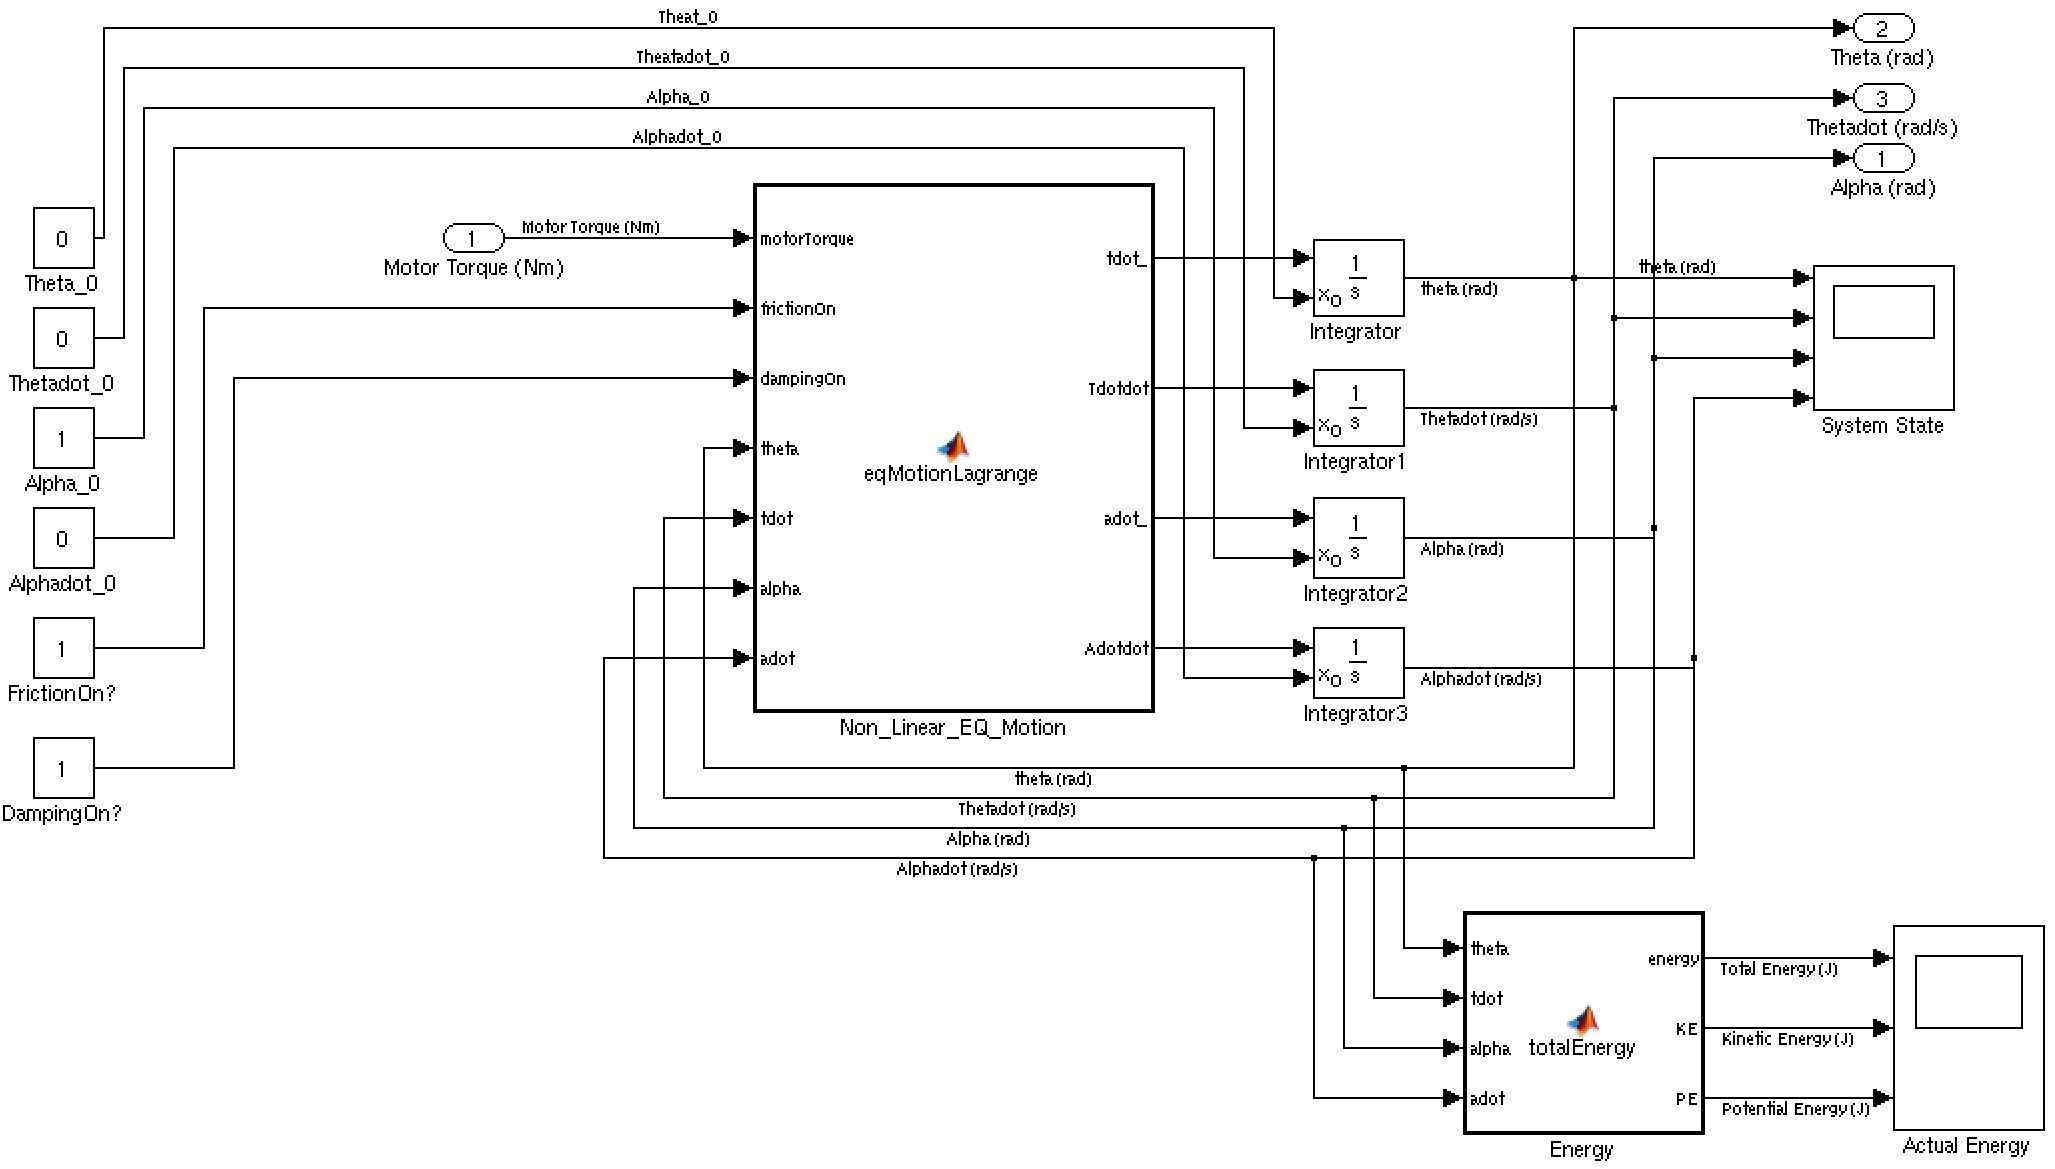
\includegraphics[width = 15cm]{NonLinearModelPic.png}
\end{center}
\caption{Block Diagram of Non-Linear System Model}
\label{NonLinearBlock}
\end{figure}

\begin{figure}
\begin{center}
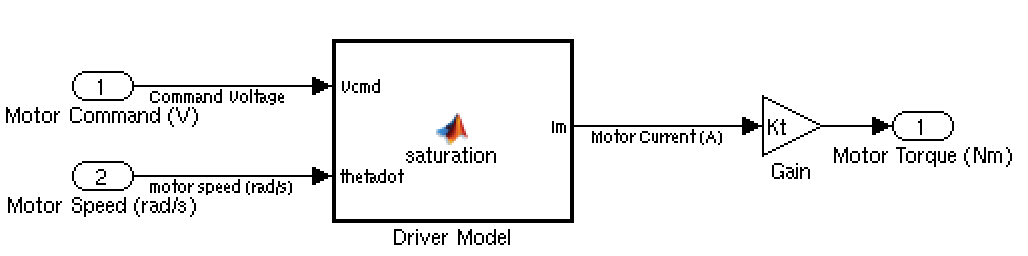
\includegraphics[width = 12cm]{DriverandMotorModel.png}
\end{center}
\caption{Block Diagram of Driver and Electrical Motor Model}
\label{DriverNonLinearBlock}
\end{figure}

\subsection*{e.}
\subsubsection*{Linearized Equations of Motion}

We will linearize the equations of motion about $\theta = 0$, $\alpha = 0$.  By taylor expansion about this point and dropping higher order terms we obtain: 

 $$ \sin(\alpha) \approx 0 \hspace{1cm} \cos(\alpha) \approx \alpha \hspace{1cm} \sin(\theta) \approx 0 \hspace{1cm} \cos{\theta} \approx \theta $$

We note that the coulomb friction terms from the previous non-linear equations must be dropped completely as there is no reasonable linearization of the effects of friction.  We also note that we expect $\dot{\theta}$ and $\dot{\alpha}$ to be relatively small, which implies: 

$$ \dot{\theta} \dot{\alpha} \approx 0 $$

Applying these to equations \eqref{NonLin1} and \eqref{NonLin2} yields \eqref{Lin1} and \eqref{Lin2} respectively.

\begin{equation}
\ddot{\theta} \left( I_{1z1} + I_{2xx} + m_2 l_1^2 \right) + \ddot{\alpha} C_3 = -b_{\theta} \dot{\theta} + \tau_{m}
\label{Lin1}
\end{equation}

\begin{equation}
\ddot{\alpha} C_1 + \ddot{\theta} C_3 - \alpha C_4 = -b_{\alpha} \dot{\alpha} 
\label{Lin2}
\end{equation}

Using equations \eqref{Lin1} and \eqref{Lin2} together we can generate two independent equations for $\ddot{\alpha}$ and $\ddot{\theta}$.

$$ C_{5} = (I_{1z1} + I_{2xx} + m_2 l_1^2) $$

\begin{equation}
\ddot{\theta} = \frac{C_3 b_{\alpha} \dot{\alpha} - C_3 C_4 \alpha - C_1 b_{\theta} \dot{\theta} + C_1 \tau_{m}}{ C_5 C_1 - C_3^2}
\label{Lin_Theta}
\end{equation}

\begin{equation}
\ddot{\alpha} = \frac{-C_5 b_{\alpha} \dot{\alpha}  + C_3 b_{\theta} \dot{\theta}  + \alpha C_4 C_5 - C_3 \tau_m }{C_5 C_1 - C_3^2}
\label{Lin_Alpha}
\end{equation}

\subsubsection*{State Space Model}

State Space Representation models a dynamical system as a set of linear, time-varying differential equations.  What is known as the state of the system is a set of variables, the generalized coordinates, $q_i$ that completely describe the internal state of the system.  For the inverted pendulum we choose the coordinates: 

$$ {\bf{X}}(t) = [q_1(t), q_2(t), q_3(t), q_4(t)]^T = [q_1(t), \dot{q}_1(t), q_3(t), \dot{q}_3(t)]^T = [\theta(t), \dot{\theta}(t), \alpha, \dot{\alpha}(t)]^T $$

In this generalized coordinate system, we compute the derivative of the state, $\dot{X}$ as a function of the current state $\bf{X}$ and the inputs $\bf{u}$. 

$$ \dot{\bf{X}(t)} = [\dot{q}_1(t), \dot{q}_2(t), \dot{q}_3(t), \dot{q}_4(t)]^T = [\dot{q}_1(t), \ddot{q}_1(t), \dot{q}_3(t), \ddot{q}_3(t)]^T = [\dot{\theta}(t), \ddot{\theta}(t), \dot{\alpha}(t), \ddot{\alpha}(t)]^T $$

Because our system is linear this relationship can be related through the State Matrix $A$ and the Input Matrix $B$ which map the current state and external inputs into the system into the change in state through the following equation.

$$ \dot{\bf{X}}(t) = A(t) {\bf{X}(t)} + B(t) {\bf{u}}(t)$$

$$ A_{ij} = \frac{\partial \dot{q}_j}{\partial q_i}(t) \hspace{1cm}  B_{i} = \frac{\partial \dot{q}_i}{\partial u_i}(t)$$

The actual output that we wish to control is determined from $\dot{\bf{X}}(t)$ and from the inputs ${\bf{u}}(t)$ through the Output Matrix, $C(t)$ and the Direct Transmission Matrix $D(t)$.  Then our output ${\bf{Y}}(t)$ can be represented as follows:

$$ {\bf{Y}}(t) = C(t) \dot{\bf{X}}(t) + D(t) {\bf{u}}(t) = C(t) \left\{ A(t) {\bf{X}(t)} + B(t) {\bf{u}}(t) \right\}+ D(t) {\bf{u}}(t)$$

As noted above the matrices A, B, C, and D may in general be functions of time, however because our system is time invariant, these matrices become independent of time.  The notation below has been simplified accordingly.  The matrices A and B may be obtained directly from our linearized equations of motion above.  

\xxx{need to format this matrix to look better}
$$ A = \left[ \begin{array}{c c c c l}
	\frac{\partial \dot{\theta}}{\partial \theta} & \frac{\partial \dot{\theta}}{\partial \dot{\theta}} & \frac{\partial \dot{\theta}}{\partial \alpha} & \frac{\partial \dot{\theta}}{\partial \dot{\alpha}}\\[6pt]
	\frac{\partial \ddot{\theta}}{\partial \theta} & \frac{\partial \ddot{\theta}}{\partial \dot{\theta}} & \frac{\partial \ddot{\theta}}{\partial \alpha} & \frac{\partial \ddot{\theta}}{\partial \dot{\alpha}}\\[6pt]
	\frac{\partial \dot{\alpha}}{\partial \theta} & \frac{\partial \dot{\alpha}}{\partial \dot{\theta}} & \frac{\partial \dot{\alpha}}{\partial \alpha} & \frac{\partial \dot{\alpha}}{\partial \dot{\alpha}}\\[6pt]
	\frac{\partial \ddot{\alpha}}{\partial \theta} & \frac{\partial \ddot{\alpha}}{\partial \dot{\theta}} & \frac{\partial \ddot{\alpha}}{\partial \alpha} & \frac{\partial \ddot{\alpha}}{\partial \dot{\alpha}}\\[6pt]
 \end{array} \right] = 
\left[ \begin{array}{c c c c l} 
0 & 1 & 0 & 0 \\
0 & \frac{\partial \ddot{\theta}}{\partial \dot{\theta}} & \frac{\partial \ddot{\theta}}{\partial \alpha} & \frac{\partial \ddot{\theta}}{\partial \dot{\alpha}} \\
0 & 0 & 0 & 1 \\
0 & \frac{\partial \ddot{\alpha}}{\partial \dot{\theta}} & \frac{\partial \ddot{\alpha}}{\partial \alpha} & \frac{\partial \ddot{\alpha}}{\partial \dot{\alpha}} \\
\end{array} \right]$$

$$ \frac{\partial \ddot{\theta}}{\partial \ddot{\theta}} = -\frac{C_1 b_{\theta}}{C_5 C_1 - C_3^2}  \hspace{1cm} \frac{\partial \ddot{\theta}}{\partial \alpha} = -\frac{C_3 C_4}{C_5 C_1 - C_3^2}
\hspace{1cm} \frac{\partial \ddot{\theta}}{\partial \dot{\alpha}} = \frac{C_3 b_{\alpha}}{C_5 C_1 - C_3^2}$$

$$ \frac{\partial \ddot{\alpha}}{\partial \dot{\theta}} = \frac{C_3 b_{\theta}}{C_5 C_1 - C_3^2} \hspace{1cm}  \frac{\partial \ddot{\alpha}}{\partial \alpha} = \frac{C_4 C_5}{C_5 C_1 - C_3^2} \hspace{1cm} \frac{\partial \ddot{\alpha}}{\partial \dot{\alpha}} = - \frac{C_5 b_{\alpha}}{C_5 C_1 - C_3^2}$$

$$ B = \left[ \begin{array}{c l} 
\frac{\partial \dot{\theta}}{\partial \tau_m} \\
\frac{\partial \ddot{\theta}}{\partial \tau_m} \\
\frac{\partial \dot{\alpha}}{\partial \tau_m} \\
\frac{\partial \ddot{\alpha}}{\partial \tau_m} \\
 \end{array} \right] 
= \left[  \begin{array}{c l} 
0 \\ \frac{C_1}{C_5 C_1 - C_3^2} \\ 0 \\ -\frac{C_3}{C_5 C_1 - C_3^2} \\
\end{array} \right] $$

We wish to stabilize the pendulum vertically, so the output be are interested in is precisely $\alpha(t)$.  Thus C becomes simply:

$$ C = [0, 0, 1, 0]^T $$

For this system, the only external input, the motor torque $\tau_{m}(t)$, does not directly influence the output, ${\bf{Y}}(t)$ except for its influence on  $\dot{\bf{X}}(t)$ making D simply the zero matrix.

$$ D = [0, 0, 0, 0]^T$$

\subsubsection*{System Transfer Functions}

To generate the transfer functions it is more straight forwards to proceed from equations \eqref{Lin1} and \eqref{Lin2} than from \eqref{Lin_Theta} and \eqref{Lin_Alpha}.  Applying the Laplace transform \eqref{Lin1} and \eqref{Lin2} yields and performing arithmetic operation to isolate $\theta (s)$ and $\alpha (s)$ yields the following transfer functions from motor torque, $ \tau (s)$ to $\theta (s)$ and $\alpha (s)$ respectively.


\begin{equation}
\frac{\theta(s)}{\tau_{m}(s)} = \frac{s^2 C_1 + s b_{\alpha} - C_4}{\left(s^2C_1 + s b_{\alpha} - C_4 \right) \left(s^2 C_5  + s b_{\theta} \right) - s^4 C_3^2}
\label{TF_Theta}
\end{equation}

\begin{equation}
\frac{\alpha(s)}{\tau_{m}(s)} = \frac{-s^2 C_3}{\left(s^2C_1 + s b_{\alpha} - C_4 \right) \left(s^2 C_5  + s b_{\theta} \right) - s^4 C_3^2}
\label{TF_Alpha}
\end{equation}

If we were to neglect the effects of damping, then \eqref{TF_Theta} and \eqref{TF_Alpha} would reduce to the following:

$$ \frac{\theta(s)}{\tau_{m}(s)} \approx \frac{s^2 C_1 - C_4}{s^2 \left[s^2 \left(C_5 C_1 - C_3^3 \right) - C_4 C_5\right]} $$

$$ \frac{\alpha(s)}{\tau_{m}(s)} \approx \frac{- s^2 C_3}{s^2 \left[s^2 \left(C_5 C_1 - C_3^3 \right) - C_4 C_5\right]} $$

In the simplified transfer function for $\alpha (s)$ above it appears as if we can cancel the $s^2$'s, but this not the case as we see when we examine equation \eqref{TF_Alpha}.  

\clearpage

\section{ Parameter Identification}
The inverted pendulum system includes many parameters related to the mechanical and electrical properties of the system. To determine these, we used a combination of manufacturer data sheets, CAD modeling, physical measurements, and experimental regression.\\

Most of the relevant motor parameters were previously determined in the DC motor lab. In that case, most of the parameters were provided by the manufacturer, but we performed regression on experimental data to fit our model with the test data and found that the true values were different from those on the data sheet. The relevant values are shown in table \ref{q2_1}. An abbreviated excerpt from our DC motor lab is given below to show our procedure for determining these values. \\

\begin{table}[htb]
\begin{center}
    \begin{tabular}{|c|c|c|}
        \hline
        ~                 & Data-Sheet Values    & Fit Values              \\ \hline
        $J_{motor} \hspace{0.1cm} \left( \frac{N \cdot s^2}{m} \right)$               & $8.5 \cdot 10^{-6} $     & $3.50514 \cdot 10^{-5}$ \\ 
        $K_{t} \hspace{0.1cm} \left( \frac{N\cdot m}{A} \right)$           & $0.0424$             & $0.0314499$             \\ 
        $b_{forwards} \hspace{0.1cm} \left( N \cdot s \right)$    & $3.7 \cdot 10^{-6} $ & $1.08586 \cdot 10^{-5}$ \\ 
        $b_{reverse} \hspace{0.1cm} \left( N \cdot s \right)$     & $3.7 \cdot 10^{-6} $ & $4.85930 \cdot 10^{-5}$ \\ 
        $\tau_{forwards} \hspace{0.1cm} \left( N \cdot m \right)$ & $5.6 \cdot 10^{-3}$  & $0.0224389$             \\ 
        $\tau_{reverse} \hspace{0.1cm} \left( N \cdot m \right)$   & $5.6 \cdot 10^{-3}$  & $0.0143096$             \\
        \hline
    \end{tabular}
\caption{DC Motor Final Parameter Values vs Original Data Sheet Values}
\label{q2_1}
\end{center}
\end{table}

To determine the parameters of the motor we used MATLAB's numerical differential equation solving to simulate the trajectory of the system as a function of time, driver current, $I_t$ and our unknown system parameters $J$, $b$, $K_t$, and $\tau_{coulomb}$.  By then
comparing the predicted angular positions with the measured angular positions over time, we can construct a non-linear regression to estimate the unknown parameters.  We collected a data set where the driver was given a sinusoidal voltage, and we assume that motor current, $I_m$, is identical to this driver voltage and recorded the motor motion that this input caused. \\

With this model and some intelligent guessing for new parameter values, we arrived at an excellent fit shown in figure \ref{q2_2}. The most notable feature of these values is the large difference between the torque of friction in the forwards and reverse directions. \\ 

\begin{figure}[htb]
\begin{center}
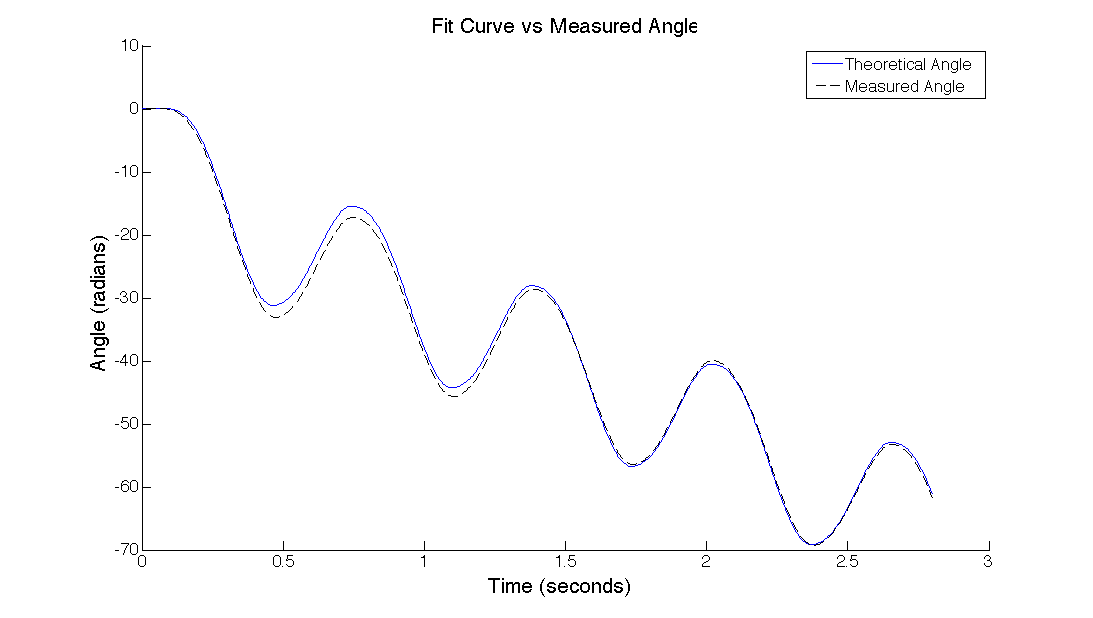
\includegraphics[width = 14cm]{awesomefitFiner.png}
\caption{Predicted behavior vs Actual behavior using fit parameter values and enhanced modeling}
\label{q2_2}
\end{center}
\end{figure}

With the motor parameters largely known already, we focused on determining the parameters of the new components comprising the pendulum and horizontal arm. To ensure accuracy, we used multiple methods and compared results. For example, the mass of every component was determined on the scale provided in the mechatronics lab. We then built CAD models of every component in SolidWorks using a combination of engineering drawings, physical measurements, and already built models from McMaster-Carr. By setting the material properties correctly, SolidWorks can determine the mass of every part. We compared this calculated value to the measured values and they all matched within the limits of resolution of the scale. This gave us confidence in the ability of SolidWorks to calculate the other necessary parameters.Therefore, we built assemblies of the pendulum, the horizontal arm and complete system, and we used SolidWorks to calculate the masses, centers of mass, and moments of inertia that we needed. Figures \ref{q2_3}, \ref{q2_4}, and \ref{q2_5} show the CAD assemblies. The inertia matrix for the pendulum and other relevant values are given below. Note that the axes labels in the SolidWorks models are not the same as those in our derived equations.

\begin{center} $ \begin{vmatrix}
\bar{I}_{xx} & \bar{I}_{xy} & \bar{I}_{xz} \\
\bar{I}_{yx} & \bar{I}_{yy} & \bar{I}_{yz} \\
\bar{I}_{zx} & \bar{I}_{zy} &  \bar{I}_{zz} \end{vmatrix}_{Pendulum}
=  \begin{vmatrix}
8.1\cdot10^{-6} & 2.03\cdot10^{-5} & 0 \\
2.03\cdot10^{-5} & 3.711\cdot10^{-4} & 0 \\
0 & 0 &  3.646\cdot10^{-4} \end{vmatrix}$\end{center}

Translating from the coordinate system established in Solid Works to our coordinate system yields the following moment of inertia tensor:

$$I_{2} = \left[ \begin{array}{c c c l} 
8.1\e{-6} & 0 & 2.03\e{-5} \\   
0 & 3.711\e{-4} & 0 \\
2.03\e{-5} & 0 & 3.646e{-4} \\
\end{array} \right] \, kg \cdot m^2$$

\begin{center}
$$m_{1} = 0.1481 kg \quad m_{2} = 0.0820 kg $$
$$ l_{1} = 0.10826 m \quad l_{2C} = 0.08568 m $$
$$I_{1zt} = \left(6.78 \e{-4} + 3.50514 \e{-5} \right) \, kg \cdot m^2 =  7.1305\cdot 10^{-4}kg\cdot m^{2}$$
\end{center}

\begin{figure}[htb]
\begin{center}
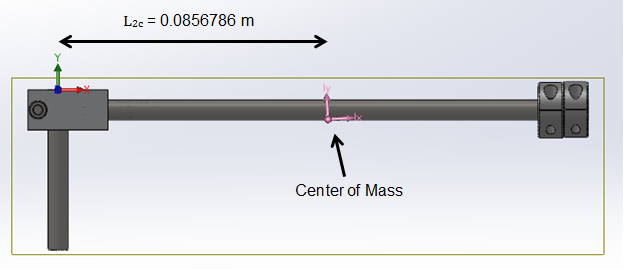
\includegraphics[width = 14cm]{PendulumModel.png}
\caption{SolidWorks Model of Pendulum}
\label{q2_3}
\end{center}
\end{figure}

\begin{figure}[htb]
\begin{center}
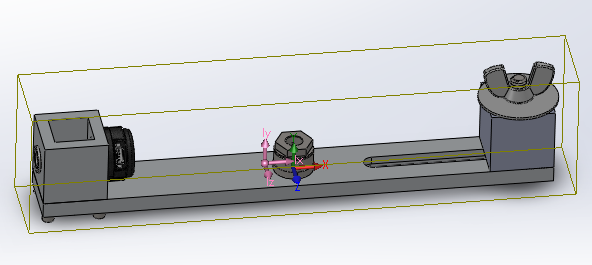
\includegraphics[width = 14cm]{Horizontal.png}
\caption{SolidWorks Model of Horizontal Link}
\label{q2_4}
\end{center}
\end{figure}

\begin{figure}[htb]
\begin{center}
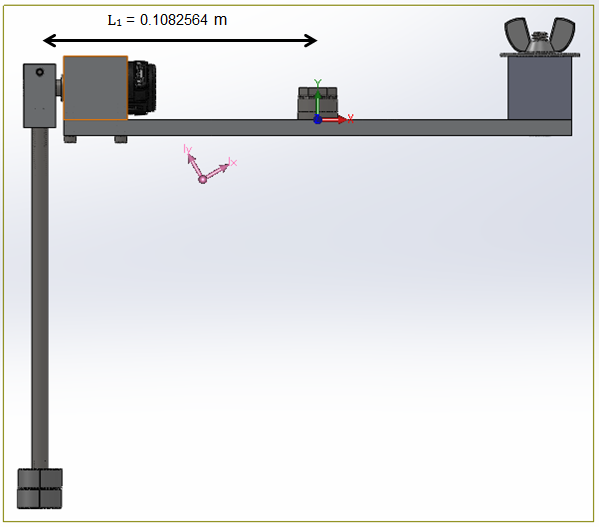
\includegraphics[width = 14cm]{CompleteArm.png}
\caption{SolidWorks Model of Assembled Pendulum and Horizontal Link}
\label{q2_5}
\end{center}
\end{figure}

For the pendulum we assume that frictional torque, $\tau_{F \alpha}$, and the viscous damping coefficient, $b_{\alpha}$ are the same in each direction. These terms for the pendulum were estimated in an experiment where the horizontal arm was fixed in place and the pendulum was allowed to swing freely from an initial angle.  By comparing the decaying envelope, extracted as the maximum and minimum of each oscillation, of the actual system motion with a similar plot generated from a simulated model, we formed a rough estimate of these terms. \\

%To determine the viscous damping and coulomb friction of the pendulum and bearings, we used non-linear regression with MATLAB's numerical differential equation solver, just as we did with the DC motor parameter identification. To do this we clamped the horizontal arm in place and allowed the pendulum to oscillate freely from several starting positions. Because of the large number of data points obtained during the time it takes the pendulum to come to rest, we extracted the peak of each oscillation for the regression instead of using every point. The damping and friction values are given below; because the friction and damping in the pendulum and bearings are so small, we assumed that they were approximately equal in both directions.\\
$$b_{\alpha} = 6.5\cdot10^{-6}\, N\cdot s \qquad \tau_{F \alpha} = 7.0\cdot10^{-6} \, N\cdot m$$

\begin{figure}
\begin{center}
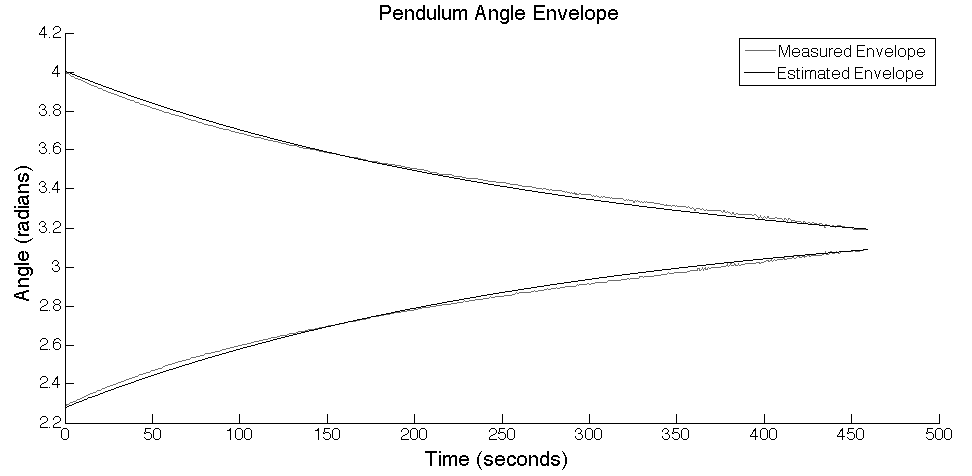
\includegraphics[width = 16cm]{pendulumEnvelope.png}
\caption{Actual Decaying Envelope of motion vs Simulated Envelope}
\label{q2_6}
\end{center}
\end{figure}

\clearpage

\section{ Comparing Linear and Non-Linear Models}
Figures \ref{q3_1} and \ref{q3_2} show the pendulum and horizontal arm angle response from the nonlinear model compared to experimental data. The data was obtained by allowing the pendulum to oscillate freely from a starting angle and then running the simulink model with the same initial conditions. The predicted pendulum angle agrees with the experimental data quite well for the first few periods, but quickly deviates. Interestingly, after several periods the experimental angle doesn't decay as quickly as the predicted angle, but the decay accelerates after several more periods and the pendulum comes to rest much sooner in the real system than in the model. A possible cause of this is the force applied by the encoder cable on the horizontal arm, which is unmodelled and very nonlinear and unpredictable. This is especially apparent in figure \ref{q3_2}, where the horizontal arm prediction and real behavior were very far off. \\

\begin{figure}[hbt]
\begin{center}
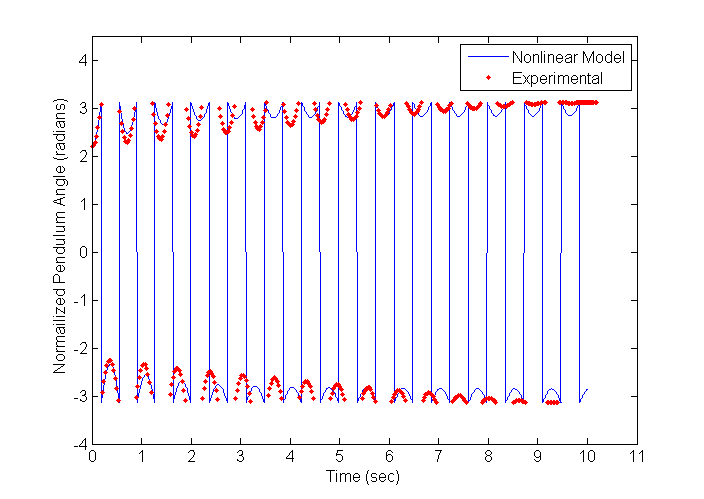
\includegraphics[width = 13cm]{alpha1.png}
\end{center}
\caption{Comparison of Normalized Pendulum Angle From the Nonlinear Model and Experimental Data}
\label{q3_1}
\end{figure}

\begin{figure}[hbt]
\begin{center}
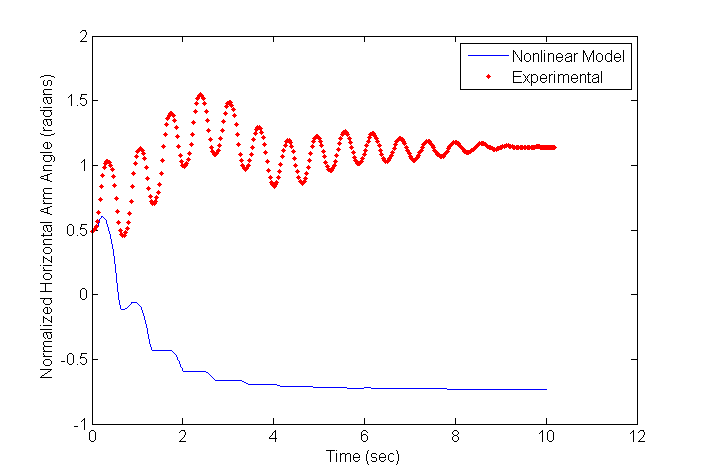
\includegraphics[width = 13cm]{theta1.png}
\end{center}
\caption{Comparison of Normalized Horizontal Arm Angle From the Nonlinear Model and Experimental Data}
\label{q3_2}
\end{figure}

Figures \ref{q3_3} and \ref{q3_4} show the pendulum and horizontal arm angle response from the linearized model compared to experimental data. The predicted pendulum angle agrees with the experimental quite well for several periods. Somewhat surprisingly, the linear model matches the experimental data longer than the nonlinear model did. However, the linear model decays extremely slowly. This is largely because the friction terms are no longer present, and friction on the horizontal arm played a large role in reducing the energy of the system. While the linear pendulum angle seems to perform reasonably well initially, the linear horizontal arm angle does not agree with the test data at all. If the angle data was not normalized, the predicted arm angle in figure \ref{q3_4} would grow without bound. A possible cause of this is that our linear model does not incorporate all of the friction and damping forces that act on the horizontal arm, and the encoder cable applies significant resistance to rotation on the arm.\\

\begin{figure}[hbt]
\begin{center}
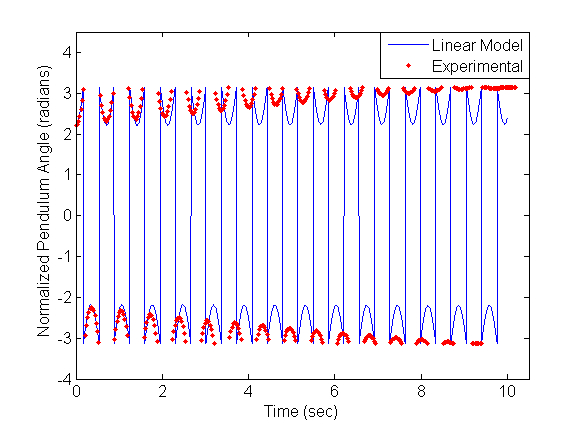
\includegraphics[width = 13cm]{alphaLinear.png}
\end{center}
\caption{Comparison of Normalized Pendulum Angle From the Linearized Model and Experimental Data}
\label{q3_3}
\end{figure}

\begin{figure}[hbt]
\begin{center}
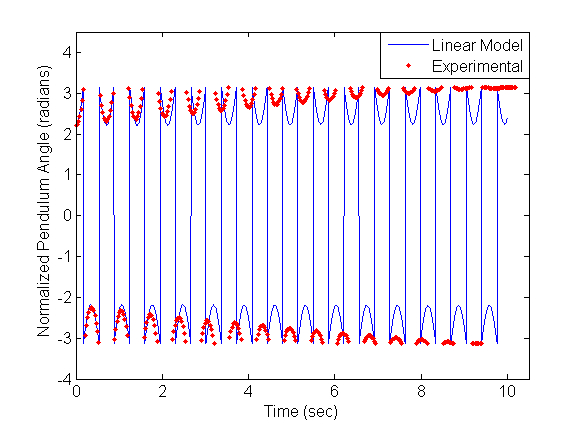
\includegraphics[width = 13cm]{alphaLinear.png}
\end{center}
\caption{Comparison of Normalized Horizontal Arm Angle From the Linearized Model and Experimental Data}
\label{q3_4}
\end{figure}

To investigate the effect that the encoder cord has on the system, we ran tests with the cable removed. This meant that we could only get data on the horizontal arm angle. To ensure consistency, we raised the pendulum to a horizontal position before releasing it, then ran the simulink model from a horizontal starting position. Figure \ref{q3_5} shows the results of such a test. The initial transient phase of the two datasets still doesn't agree, and the real system decays much slower, but it's interesting that both move towards +-$\pi$ (though the normalization of the angles makes this somewhat hard to see). This suggests to us that the cord is having a large effect on the system, but there are other factors which haven't been considered (such as tilt of the table).\\

\begin{figure}[hbt]
\begin{center}
\includegraphics[width = 13cm]{thetaNoCord.png}
\end{center}
\caption{Comparison of Normalized Horizontal Arm Angle From the Nonlinear Model and Experimental Data with the Encoder Cable Removed}
\label{q3_5}
\end{figure}

Figure \ref{q3_6} shows the predicted pendulum angle from the nonlinear model and from the linearized model. Just as when comparing both models to the experimental data, there is some agreement in the first few periods, but then the two models diverge. This is largely because the lack of friction in the linearized model causes it to decay much more slowly. There is also a noticeable phase difference as time increases because the nonlinear model predicts a slightly longer period of oscillation. \\

It is clear that there are weakness in the linear model based on the weak agreement with the nonlinear model and real system. However, this is largely because the linearization assumptions are based on the pendulum being very close to the vertical equilibrium point for use with a balancing controller. While we linearized the system about the bottom position for the purposes of comparing to the test data, the assumptions that the small angle theorem would hold and that $\dot{\theta}$ and $\dot{\alpha}$ would be small were not necessarily true when in a free swinging situation instead of being balanced. Therefore, we believe that our linearization assumptions are valid as long as we only apply the linearization within a small angle range and have a balance controller active to minimize $\dot{\theta}$ and $\dot{\alpha}$. The greatest effect of the linearization was the dropping of the friction terms (which was more of a practical necessity rather than an assumption). This had a large effect on the decay of the systems oscillations, but with our balance controller active, this assumption should not have a significantly negative effect.\\

\begin{figure}[hbt]
\begin{center}
\includegraphics[width = 13cm]{linearAndNonlinear.png}
\end{center}
\caption{Comparison of Normalized Pendulum Angle From the Nonlinear Model and Linearized Model}
\label{q3_6}
\end{figure}


\clearpage
\section{State Space Controls in Simulink}



Using the $A$, $B$, $C$, and $D$ matrices derived earlier together with the tuned $Q$ and $R$ matrices below, we constructed a full-state feedback controller using the Matlab $lqr$ function.  
$$Q = \left[\begin{array}{c c c c l} 10 & 0 & 0 & 0 \\ 0 & 40 & 0 & 0 \\ 0 & 0 & 120 & 0 \\ 0 & 0 & 0 & 60 \\  \end{array} \right] \hspace{1cm} R = \left[ 6 \right]$$

\begin{figure}[hbt]
\begin{center}
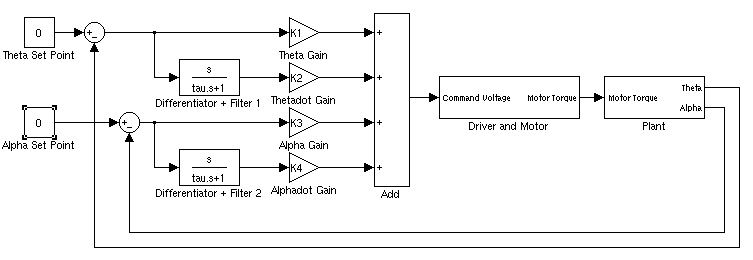
\includegraphics[width = 16cm]{stateSpaceFeedbackBlock.png}
\end{center}
\caption{Block Diagram of State Space Balancing Controller}
\label{StateSpaceBlock}
\end{figure}

$$ K_1 = -1.2910 \hspace{1cm} K_2 = -2.9161 \hspace{1cm} K_3 = -66.3961 \hspace{1cm} K_4 = -8.4496 $$

The full-state feedback controller using the gains above successful stabilized both of our linear and non-linear models.  The effects of disturbing the system with an angle of $0.1$ radians is shown in figures \ref{LvsNonLwoutF} and \ref{LvsNonLwF}.  Figure \ref{LvsNonLwoutF} compares the response of the linear system to the response of the non-linear model.  The most obvious difference between both responses is the significantly larger oscillations present in the linear system although each system shows similar behavior.  We note in the $\alpha$ response that the linear model overshoots the set point angle before returning to the set point angle over a long period of about $0.6$ seconds.  The non-linear model on the other hand shows very little overshoot at all and settles in under $0.2$ seconds.  However the controller has difficulty returning $\theta$ to the set point in the non-linear model taking approximately 10 seconds to return to $0$. 

Figure \ref{LvsNonLwF} introduces frictional forces to the non-linear model.  Here we note that the system remains stable, but $\theta$ is unable to return to its set-point settling at $0.545$ radians after about $10$ seconds.  

\begin{figure}
\begin{center}
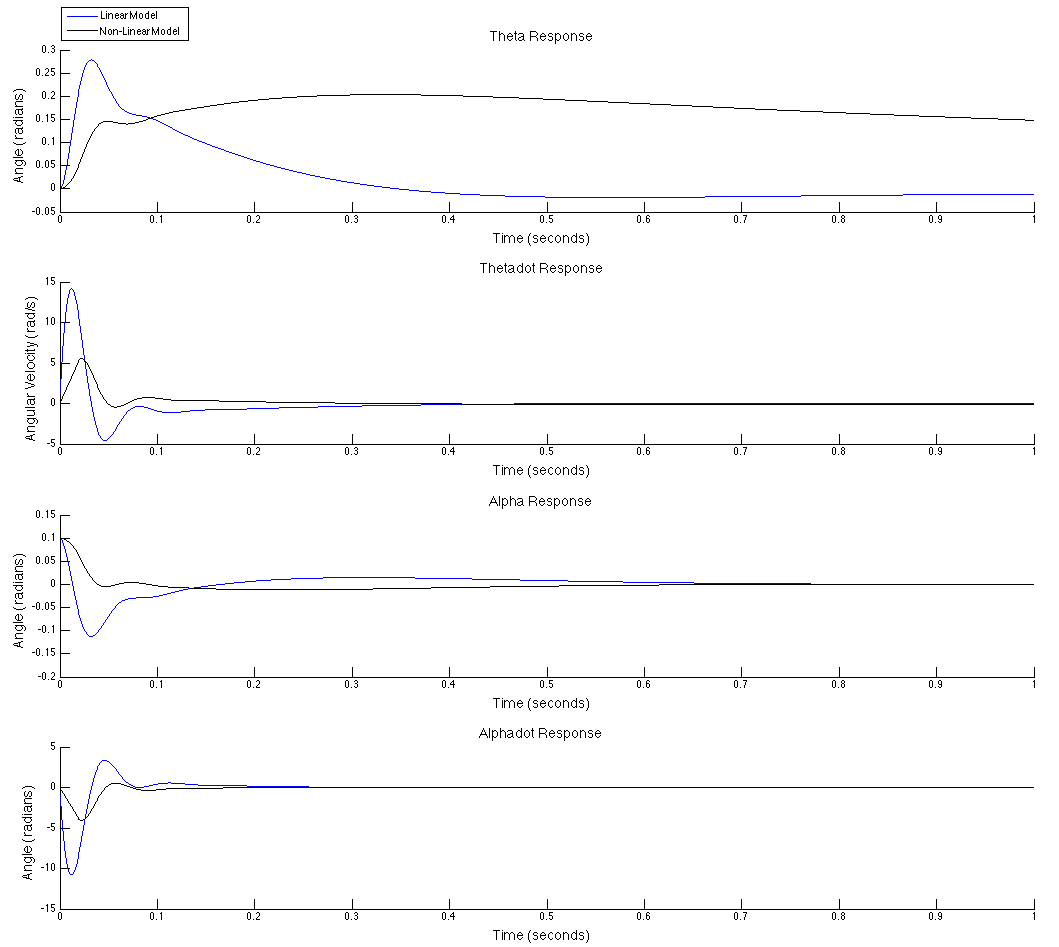
\includegraphics[width = 16cm]{nonlinearvslinearwoutF.png}
\end{center}
\caption{Comparison of Balancing controller response to perturbation, $\alpha_0 = 0.1$, for Linear and non-Linear models}
\label{LvsNonLwoutF}
\end{figure}

\begin{figure}
\begin{center}
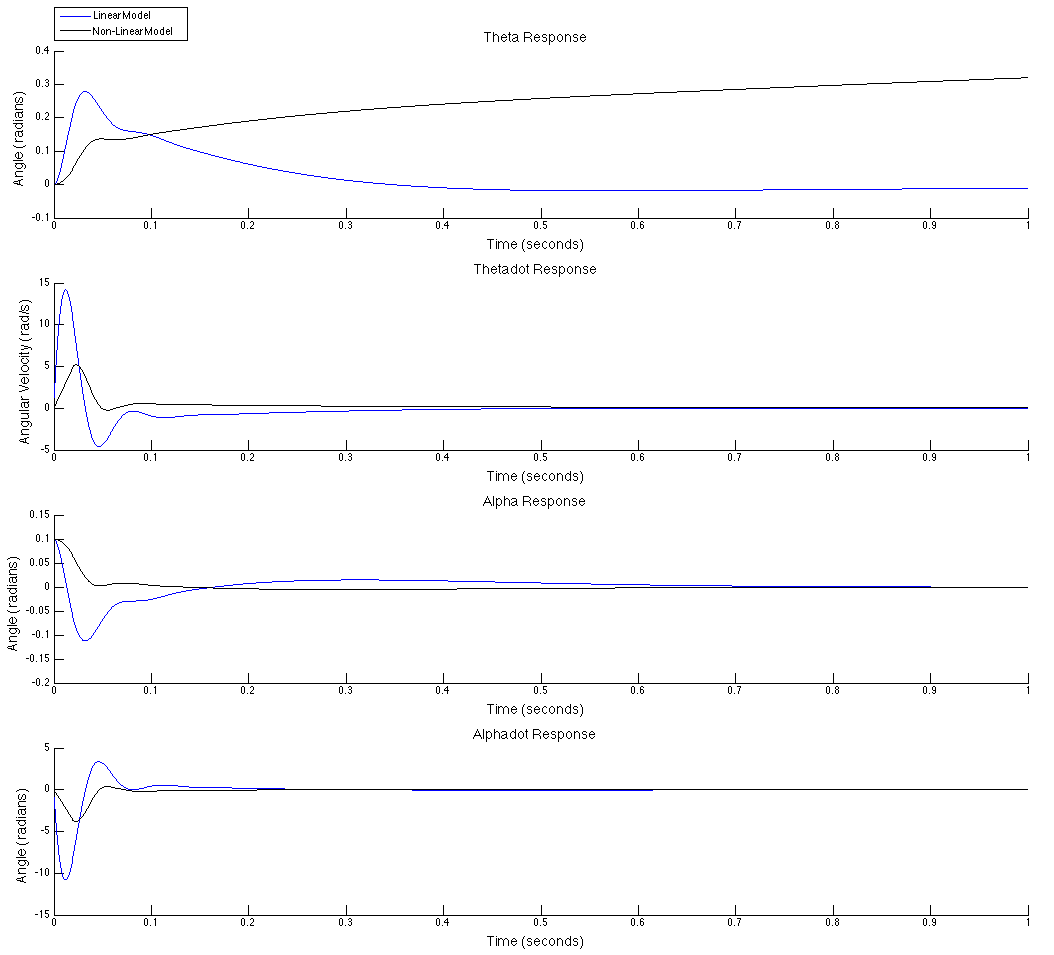
\includegraphics[width = 16cm]{nonlinearvslinearwF.png}
\end{center}
\caption{Comparison of Balancing controller response to perturbation, $\alpha_0 = 0.1$, for Linear and non-Linear models including effects of friction in the non-Linear Model}
\label{LvsNonLwF}
\end{figure}

\clearpage
\section{Swing Up Controller in Simulink}

The objective of the swing-up controller is to provide the pendulum enough energy to allow the it to reach the top position where it's potential energy is maximized.  Fig.~\ref{fig:q5_1} shows the overall scheme of the swing-up controller. This design follows the equation provided in the lecture slides: V=Ka(E-Eo)sgn(d$\alpha$/dt cos$\alpha$). $E_{set}$ is set to 0 which represented the desired total energy, and E is the total energy consisting of the kinetic and potential energy of both motor and pendulum arms.  Fig.~\ref{fig:q5_2} shows the switching mechanism between the balancing controller and the swing-up controller. Both controllers have four main inputs:  $\alpha$, $\dot{\alpha}$, $\theta$, $\dot{\theta}$, and the balancing controller has two additional inputs including the equilibrium points of $\alpha$ and $\theta$. The lead filters used to estimate the derivatives of $\theta$ and $\alpha$ introduce some lag into $\dot{\theta}$ and $\dot{\alpha}$.  Without compensation this causes the estimates of kinetic energy and potential energy to be out of phase with one another resulting in an incorrect energy total.  To compensate, we applied the same lag to the $\theta$ and $\alpha$ channels.  We use the angle $\alpha$ to determine when to switch from the swing up controller to the balancing controller described earlier. The swing-up controller shuts off at $0.45 \, radians$ and the balancing controller activate at $0.35 \, radians$.  The dead-band of 0.1 rad, provides a buffer for the pendulum to decrease its speed so that the balancing controller could catch it more easily.\\
\begin{figure}[b!]
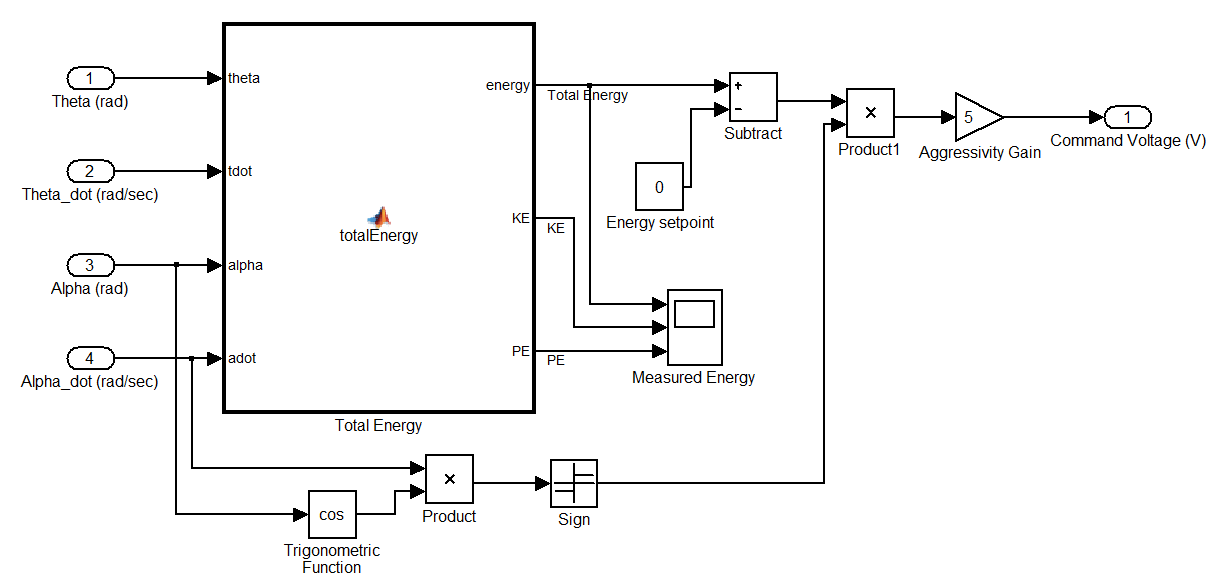
\includegraphics[width=1\textwidth]{q5_1.png}
\caption{Swing-up and Balancing Controllers with a Switching Mechanism} \label{tex}
\label{fig:q5_1}
\end{figure}

\begin{figure}[h!]
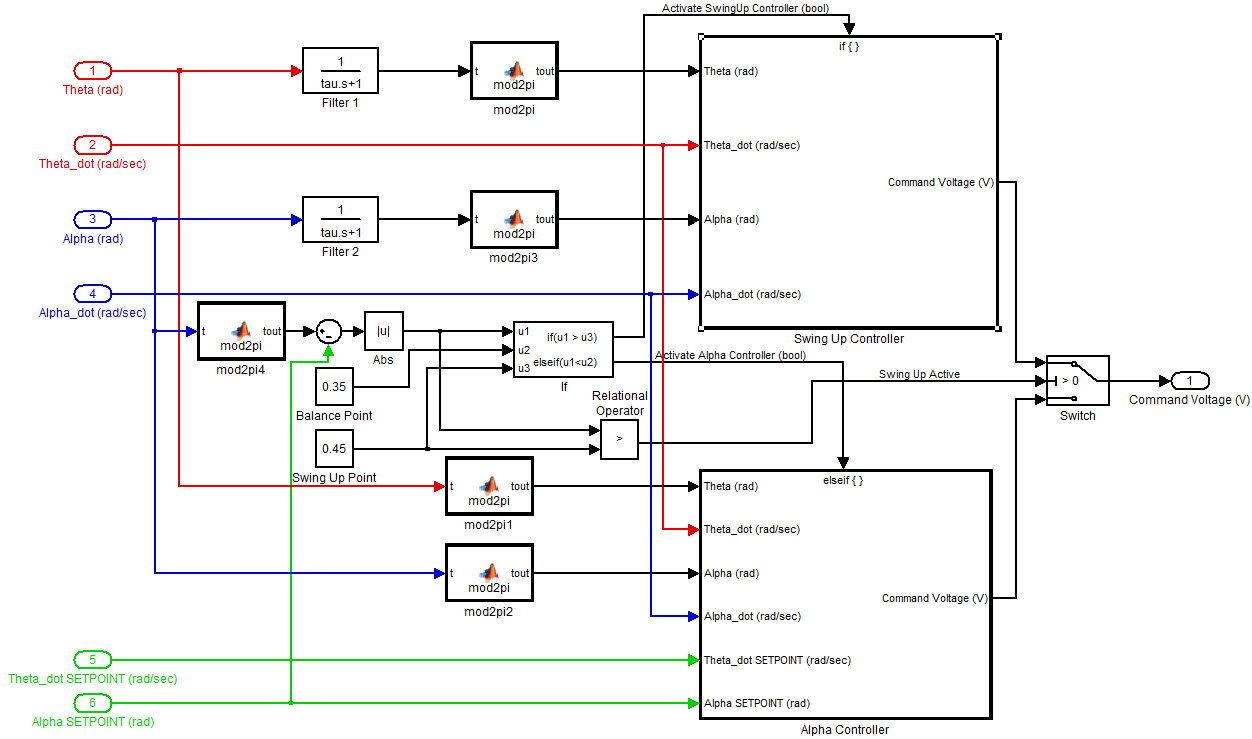
\includegraphics[width=1\textwidth]{q5_2.png}
\caption{Swing-Up Controller} \label{tex}
\label{fig:q5_2}
\end{figure}

Fig.~\ref{fig:q5_3} and~\ref{fig:q5_4} show the simulation results for two different initial conditions (3.14 rad, 0.5 rad) of $\alpha$ with the aggressive gain equal to 6. As we can see in both conditions, it takes less than 3 seconds to reach the steady state. The one with IC=3.14 required 4 swings to reach the balancing range, while the other one with IC=0.5 even achieved the goal in 1 second since it had more potential energy at the beginning.\\

We have added two additional features to our swing up controller beyond the original specification.  The first is a mechanism to reasonably convert from the energy error produced by the difference of the total energy to a command.  We can estimate the amount of energy that will be imparted to the system by applying a particular torque.  
$$ Work = \tau \cdot \delta \theta \approx \tau \cdot \dot{\theta} \cdot \Delta time $$
The other additional feature is an alternate system to reduce system energy when it exceeds the set point.  The default swing up controller can get trapped in a cycle where it continues to add more energy because it has too much energy.  For $|\alpha| > \frac{\pi}{2}$ and $\dot{\alpha} > 0$ we would normally swing increase $\dot{\alpha}$ however, if we have too much energy we will attempt to decrease $\dot{\alpha}$ by increasing $\dot{\theta}$.  When $\dot{\alpha}$ is negative we will do the opposite and the system can become trapped in a loop where the horizontal arm is rotating rapidly.  
The net result of these additional features is that the system performed even much better than the previous one. As shown in Fig.~\ref{fig:q5_6}, the pendulum reaches the balancing steady-state with only one swing.       


\begin{figure}[h!]
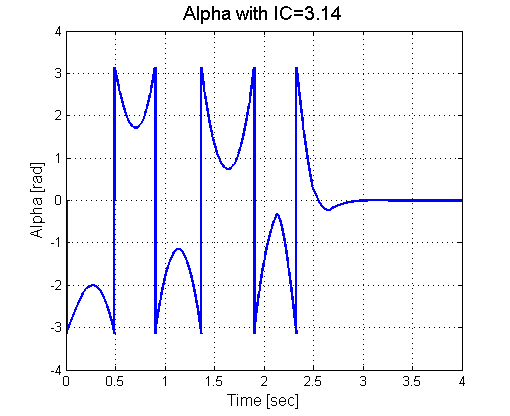
\includegraphics[width=1\textwidth]{q5_3.png}
\caption{Behavior of $\alpha$ with IC=3.14 rad} \label{tex}
\label{fig:q5_3}
\end{figure}

\begin{figure}[h!]
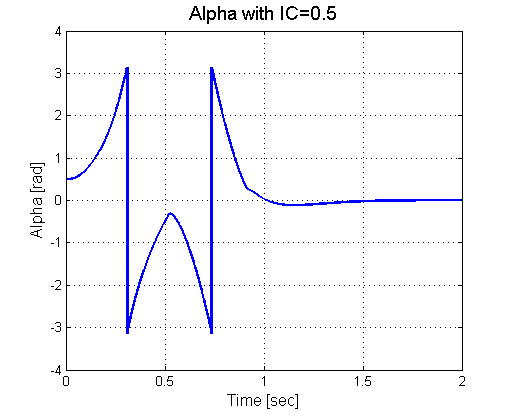
\includegraphics[width=1\textwidth]{q5_4.png}
\caption{Behavior of $\alpha$ with IC=0.5 rad} \label{tex}
\label{fig:q5_4}
\end{figure}

\begin{figure}[h!]
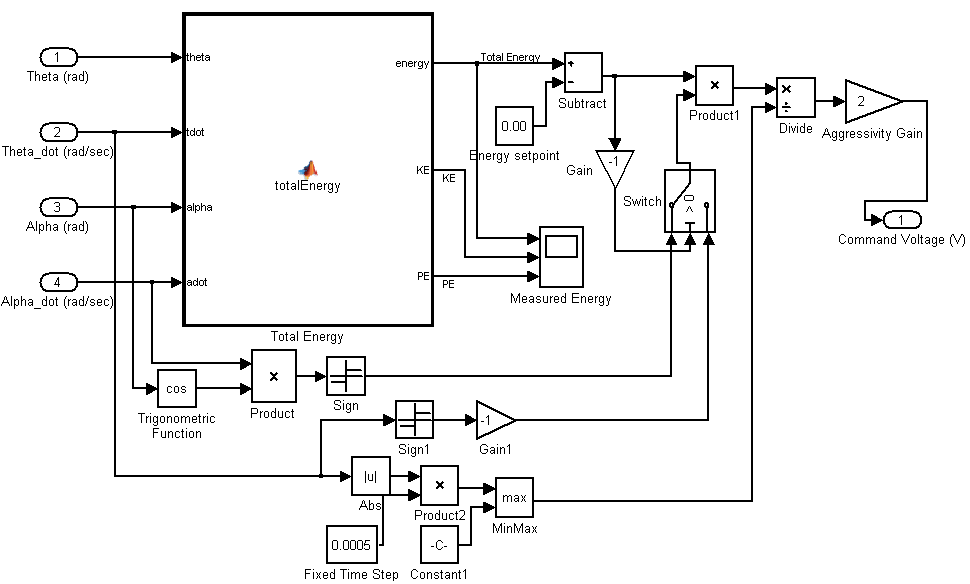
\includegraphics[width=1\textwidth]{q5_5.png}
\caption{Swing-Up Controller with Energy-Limit Mechanism} \label{tex}
\label{fig:q5_5}
\end{figure}

\begin{figure}[h!]
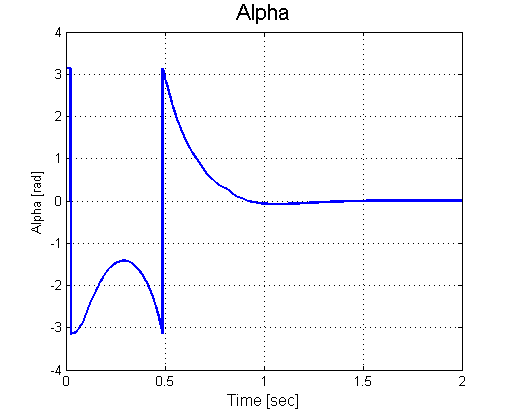
\includegraphics[width=1\textwidth]{q5_6.png}
\caption{Behavior of $\alpha$ with IC=3.14 rad} \label{tex}
\label{fig:q5_6}
\end{figure}

\clearpage
\section{LabView Implementation}

\subsection*{a.}
Angle normalization was implemented using the $mod2\pi()$ function. The function works by limiting an input angle, $\theta$ to $\pm \pi $ radians which effectively represents the entire angular spectrum of $2\pi$ radians. The advantage of using $mod2\pi()$ over a function that normalizes $\theta$ from $0$ to $2\pi$ is that the angular reset point is at $\pm \pi$ as opposed to $0$ radians. For our inverted pendulum we would like to ensure that $\alpha$ and $\theta$ are close to zero. Using $mod2\pi()$ ensures that spikes do not occur about the transition point.\\

The code for the $mod2\pi()$ operation is as follows:

\begin{verbatim}
if t<0
    t = -t;
    sign = -1;
else
    sign = 1;
tout = sign*(t - floor(t*0.5/pi + 0.5) * 2 *pi);
\end{verbatim}

In the code above $t$ represents $\theta$. For our normalization, we require $t$ to be positive and we keep track of the original sign of $t$ through the variable $sign$. $tout$ represents the output value of $mod2\pi(\theta)$ . The $floor$ operation essentially finds the quotient of dividing $t$ by $2\pi$ and the the $+ 0.5$ operation allows the angle to be normalized between $+\pi$ on one side and $-\pi$ on the other. This way, we can constrain $\theta$ to stay between $\pm \pi$.\\

$mod2\pi$ is very useful for controlling $\alpha$. $\alpha$ will reach its unstable equilibrium every $2\pi$ radians and we are happy with it as long as the pendulum balances in the unstable equilibrium. Additionally the change from $+\pi$ to $-\pi$ occurs when the the pendulum is facing downwards, but at this point the swing-up controller would be operational and for the swing-up controller, the sign of $\cos(\alpha)$ in the $+\pi$ and $-\pi$ quadrants are the same, so this does not affect the system.\\

For $\theta$ control we have to be a little careful - the horizontal arm moves a lot during swing up and generally during balancing as well, if we apply a $mod2\pi()$ operation before calculating $\dot{\theta}$, the derivative will spike up violently during the $\pm \pi$ crossover point - this in turn would destabilize the inverted pendulum system. Hence it is a good idea to calculate $\dot{\theta}$ from $\theta_{\text{Absolute}}$.\\

In general it is good practice to use a $mod2\pi()$ operation on repetitive angular functions, it helps in numerical precision in trigonometric functions and also captures the nature of the system - after a point, we get back to where we were.\\

While implementing the system in Labview we used the Matlab script block which allowed us to write Matlab code for execution as opposed to creating a messy wire-block diagram. The front panel and the block diagram can be seen in figure \ref{q6_a}.

\begin{figure}[htb]
\begin{center}
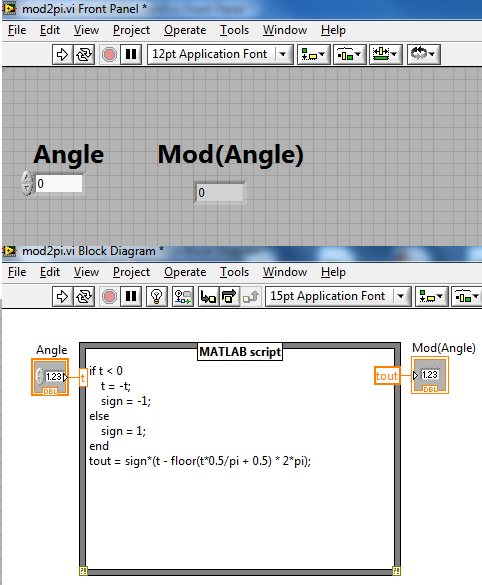
\includegraphics[width = 8cm]{q6_a.png}
\end{center}
\caption{Front panel and block diagram of $mod2\pi$.}
\label{q6_a}
\end{figure}

\clearpage

\subsection*{b.}

Figures \ref{q6_b2} through \ref{q6_b8} show the various front panels and block diagrams of the various VIs and subVIs that make up the LabView controllers.


\begin{figure}[htb]
\begin{center}
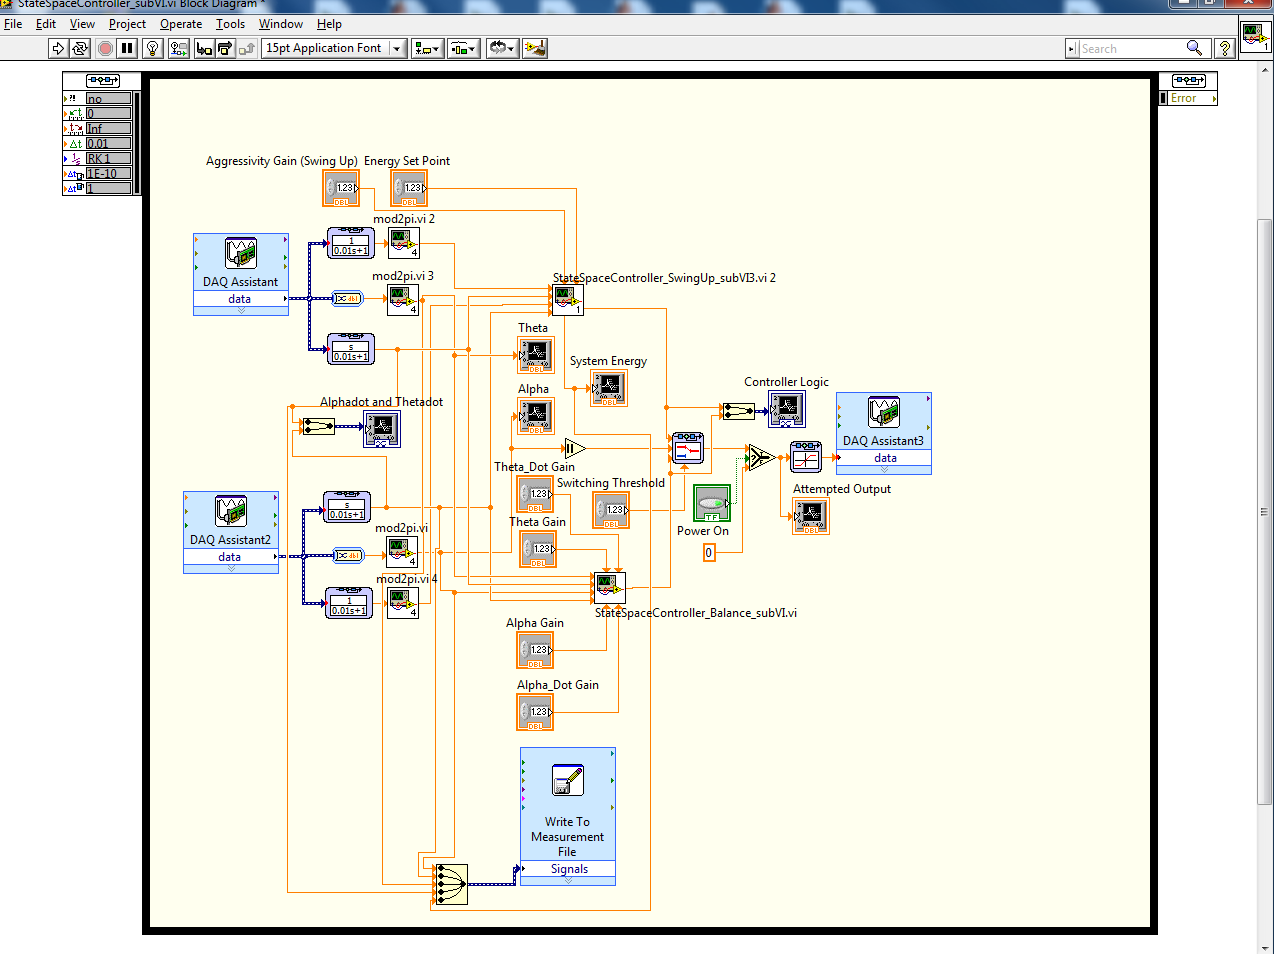
\includegraphics[width = 16cm, height = 14cm]{q6_b2.png}
\end{center}
\caption{Block diagram of State-Space Controller VI.}
\label{q6_b2}
\end{figure}


\begin{figure}[htb]
\begin{center}
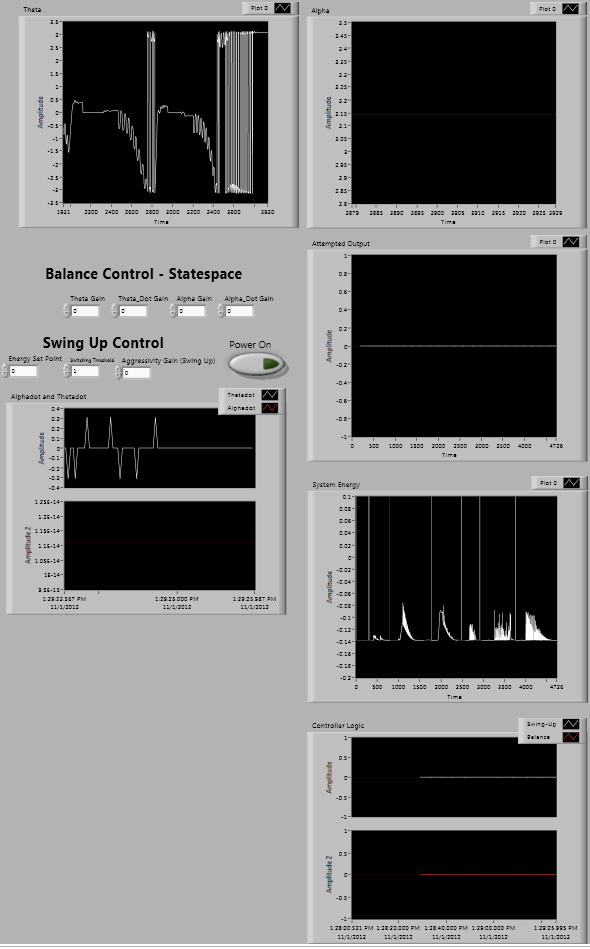
\includegraphics[width = 12cm]{q6_b1.png}
\end{center}
\caption{Front panel of State-Space Controller VI.}
\label{q6_b1}
\end{figure}




\begin{figure}[htb]
\begin{center}
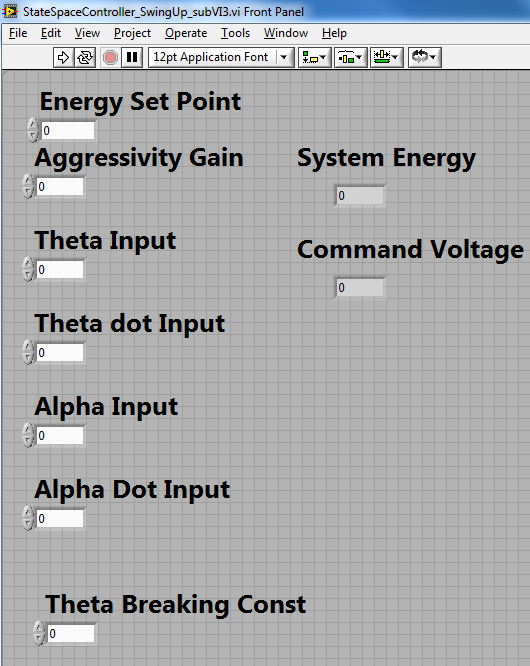
\includegraphics[width = 12cm]{q6_b3.png}
\end{center}
\caption{Front panel of the swing up controller. The \emph{Theta Breaking Constant} is used to limit the excessive overshoot of the pendulum - this could happen during swing-up or even if someone adds excessive energy to the system by tapping the pendulum very aggressively. The theta breaking algorithm attempts to move the motor in such a way that it opposes movement in $\theta$, this would dissipate excessive energy from the system.}
\label{q6_b3}
\end{figure}


\begin{figure}[htb]
\begin{center}
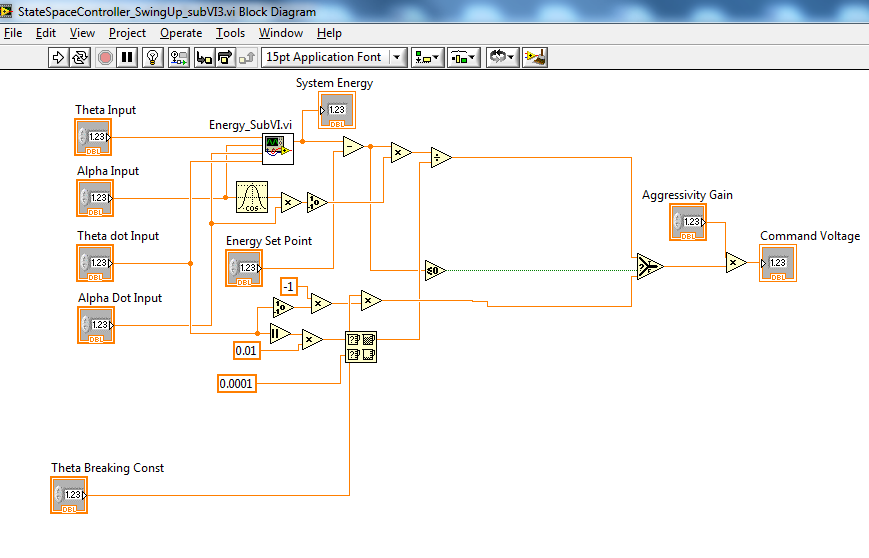
\includegraphics[width = 16cm, height = 12cm]{q6_b4.png}
\end{center}
\caption{Block diagram of the swing up controller. Theta breaking is achieved by pulsing in the opposite direction of $\theta$. The magnitude is manually tuned. If it is too high, it would inevitably add energy to the system, too small and it does not make a difference. The best hand tuned value was found to be 1.}
\label{q6_b4}
\end{figure}


\begin{figure}[htb]
\begin{center}
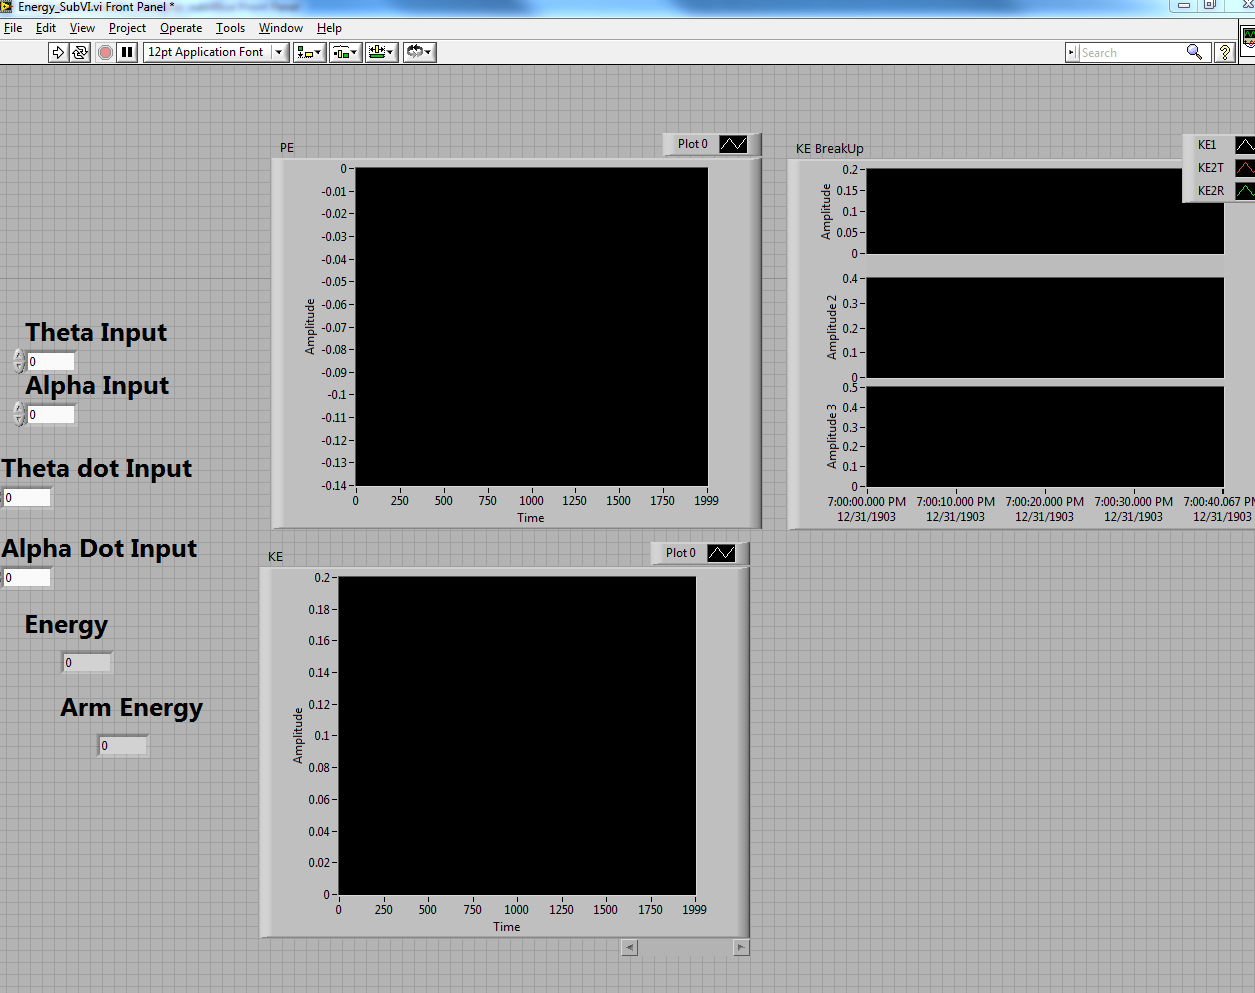
\includegraphics[width = 9cm]{q6_b5.png}
\end{center}
\caption{Front panel energy calculation subVI.}
\label{q6_b5}
\end{figure}


\begin{figure}[htb]
\begin{center}
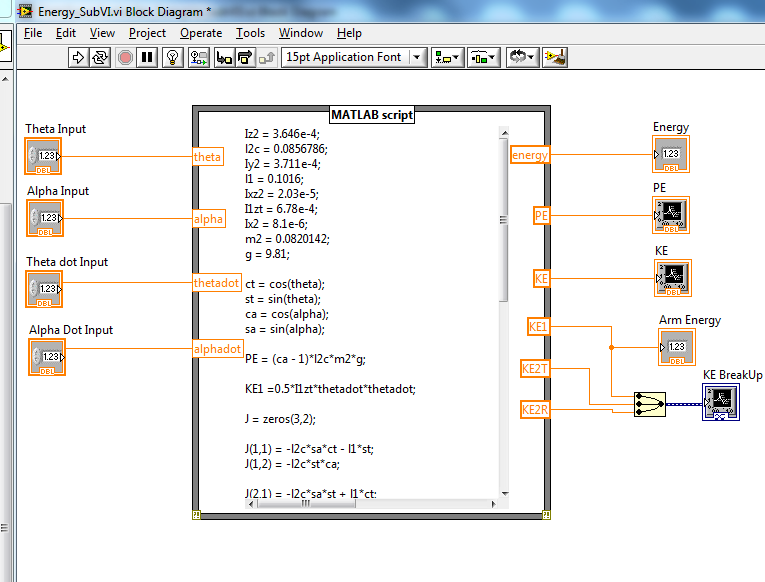
\includegraphics[width = 14cm]{q6_b6.png}
\end{center}
\caption{Block diagram of the energy calculation subVI. We used the Matlab script block again to aide in the writing the complicated equations instead of using block-based logic. The code is available in the Appendix.}
\label{q6_b6}
\end{figure}


\begin{figure}[htb]
\begin{center}
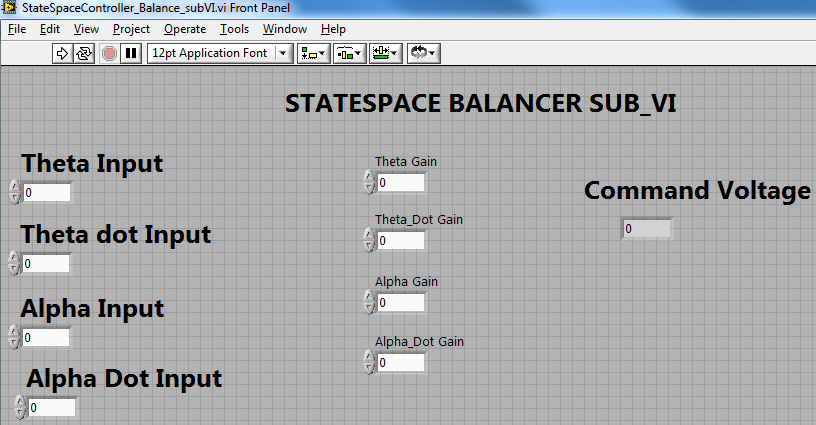
\includegraphics[width = 10cm]{q6_b7.png}
\end{center}
\caption{Front panel of the State Space Controller.}
\label{q6_b7}
\end{figure}


\begin{figure}[htb]
\begin{center}
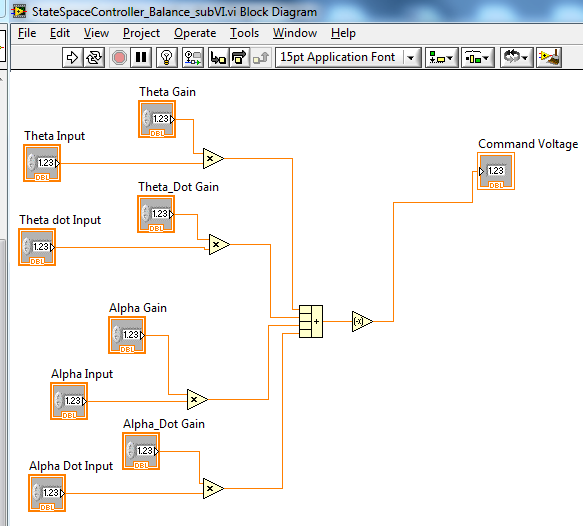
\includegraphics[width = 14cm]{q6_b8.png}
\end{center}
\caption{Block diagram of the State Space Controller.}
\label{q6_b8}
\end{figure}

\clearpage

\subsection*{c.}
For the comparison of the actual system with the simulink model, we positioned the pendulum at $\alpha = 0.2$ radians so that the balance controller could grab the pendulum and balance it. A comparison between the predicted response and actual response can be seen in figure \ref{q6_c_alpha} and \ref{q6_c_theta}. 0.1 seconds of lag can be accounted for the delay we purposefully introduced in $\alpha$ and $\theta$ so that they are in phase with $\dot{\alpha}$ and $\dot{\theta}$. This minor introduction of lag helps stabilize the system better as the angle will not lead the angular velocity. Other delays and discrepancies can be attributed to unmodeled  system properties, unaccounted motor inertia and external disturbances.\\

 The trends for $\alpha$ (theoretical and observed) seem similar and the predicted model closely resembles the real system. However, for $\theta$, we see a considerable gap in the prediction v.s. the actual behavior. We attribute these differences to the fact that we manually lifted the pendulum up to $\alpha = 0.2$ radians - which was an imperfect operation, which in itself changes the initial starting condition for $\theta$. When combined with the fact that we are more interested in holding $\alpha$ at zero, the system will stabilize $\alpha$ much faster than $\theta$.



\begin{figure}[htb]
\begin{center}
\includegraphics[width = 16cm]{Q6_C_Alpha.png}
\end{center}
\caption{Alpha response during balancing - theoretical v.s. actual}
\label{q6_c_alpha}
\end{figure}

\begin{figure}[htb]
\begin{center}
\includegraphics[width = 16cm]{Q6_C_Theta.png}
\end{center}
\caption{Theta response during balancing - theoretical v.s. actual}
\label{q6_c_theta}
\end{figure}

\clearpage

\subsection*{d.}

Table \ref{q6_d_tab} shows the results for testing the system under various conditions. Distances were measured using a vernier caliper between the outer edges of the objects and the closest part of the pendulum's body. For the counter-weight, this was between the weight and the keyless bushing and for the pendulum masses, it was between the weight mounted lowest on the shaft to the aluminum connector.\\

We noticed that the system performed robustly for major changes in the system. The only point where it could not swing up was when the masses were mounted \emph{much} lower than usual. We attribute this to the fact that the system is unable to accurately estimate the energy of the system and to the fact that our motor was not strong enough to swing up at that point.

\begin{table}[htb]
\begin{center}
    \begin{tabular}{|p{2.5cm}||p{3cm}|p{2cm}|p{2.5cm}|p{6cm}|}
        \hline
        \textbf{System}                        &\textbf{ Property}                           & \textbf{Value /}               & \textbf{Observations}                        & \textbf{Comments}                                                                                                 \\ 
        \textbf{Configuration}                 & ~                                  & \textbf{Position}              & ~                                   & ~                                                                                                        \\ \hline \hline
        Standard                      & Counter Weight position            & 67.45 mm              & Normal                              & -                                                                                                        \\ \hline
        ~                             & Pendulum Mass                      & 2 weights at 135.41mm & Normal                              & -                                                                                                        \\ \hline \hline
        Modifying Weights             & No Counter Weight                  & -                     & Swings up and balances              & Shudders more, this could be due to less inertia.                                                        \\ \hline
        ~                             & No pendulum mass                   & -                     & Swings up and balances              & Had to increase aggressivity, balancing is slightly shaky                                                \\ \hline
        ~                             & No pendulum mass or Counter Weight & -                     & Swings up and balances              & Had to increase aggressivity, balancing is VERY shaky                                                    \\ \hline \hline
        Modifying the Pendulum Masses & 1 mass                             & End of pendulum       & Swings up and balances              & No noticeable change                                                                                     \\ \hline
        ~                             & 2 masses                           & 32.52 mm              & Able to balance, unable to swing up & Energy calculations could be off: system thinks it has more Energy than it does. Also our motor is weak \\ \hline\hline
        Modifying the Counter Weight  & ~                                  & 10.16 mm              & Swings up and balances              & Slow swing up due to higher inertia on motor                                                             \\
        \hline \hline
    \end{tabular}
\end{center}
\caption{Emperical results of various configurations to test system robustness}
\label{q6_d_tab}
\end{table}

\clearpage
\section{Effects of LabView Loop Rate on Stability}
We ran the system at a loop rate of 0.01 seconds (100 Hz) and tuned our filter to reject noise at this rate. We had satisfactory system robustness and additionally, we were able to use stronger low pass filters to reject more noise.\\

In order to test the limits of stability, we changed the loop rate logarithmically. As we can see from table \ref{q7}, there is a lower bound and an upper bound for the limits of stability. We can attribute the lower bound to the fact that our filters were not designed to operate at such high frequencies. The upper bound stability loss is attributed to the inability of the system to respond quickly enough to balance the system or capitalize on the swinging the pendulum in the opposite direction to lift it up.
\begin{table}[htb]
\begin{center}
    \begin{tabular}{|c|c|}
        \hline
        \textbf{Loop Rate}(sec) & \textbf{Comment}\\ \hline\hline
        0.003     & \emph{Balancing doesn't work} \\ \hline
        0.004     & \emph{Swing Up doesn't work } \\ \hline
        0.005     & Both work                    \\ \hline
        0.006     & Both work                    \\ \hline
        0.007     & Both work                    \\ \hline
        0.008     & Both work                    \\ \hline
        0.009     & Both work                    \\ \hline
        0.01      & Both work                    \\ \hline
        0.02      & \emph{Both Fail}             \\
        \hline
    \end{tabular}
\end{center}
\caption{Emperical results of various configurations to test system robustness}
\label{q7}
\end{table}


\section{Classical Controller}

In addition to State Space Controls as detailed earlier in this report we can also attempt to apply our classical controls knowledge to design a controller in the Laplace domain.  The transfer functions of the system, $G_1(s)$ and $G_2(s)$ between motor torque, $\tau_m(s)$, $\theta(s)$ and  $\alpha(s)$ respectively computed earlier are repeated below.  As mentioned earlier, it is necessary to consider the effects of damping as they serve to make the system less, rather than more stable.  

\begin{equation}
 G_1(s) = \frac{\theta(s)}{\tau_{m}(s)} = \frac{s^2 C_1 + s b_{\alpha} - C_4}{\left(s^2C_1 + s b_{\alpha} - C_4 \right) \left(s^2 C_5  + s b_{\theta} \right) - s^4 C_3^2}
\label{thetaTF1}
\end{equation}

\begin{equation}
G_2(s) = \frac{\alpha(s)}{\tau_{m}(s)} = \frac{-s^2 C_3}{\left(s^2C_1 + s b_{\alpha} - C_4 \right) \left(s^2 C_5  + s b_{\theta} \right) - s^4 C_3^2}
\label{alphaTF2}
\end{equation}

\begin{figure}[hbt]
\begin{center}
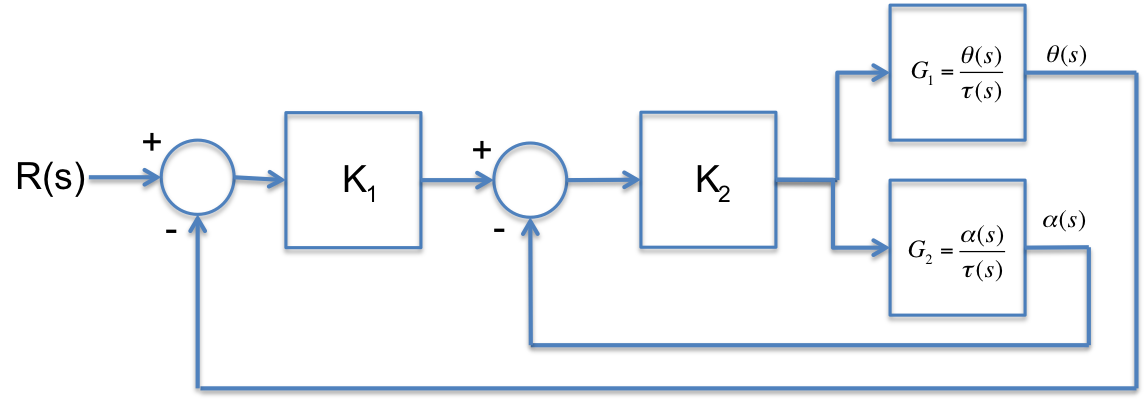
\includegraphics[width = 15cm]{classicalBlockDesign.png}
\end{center}
\caption{Block Diagram of Classical Balancing Controller}
\label{classicalControllerBlock}
\end{figure}

\begin{figure}[hbt]
\begin{center}
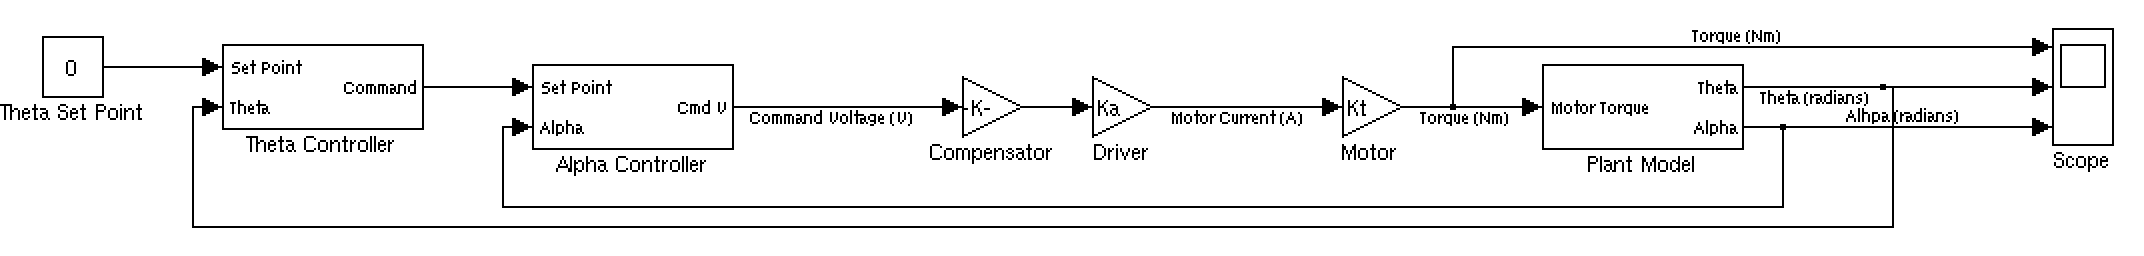
\includegraphics[width = 17cm]{ClassicalControllerBlock.png}
\end{center}
\caption{Loop within a loop to control both $\theta$ and $\alpha$ in Simulink Model}
\label{classicalSimulink}
\end{figure}

Because we have two coupled output variables that we wish to control, $\theta(s)$ and $\alpha(s)$ and only a single input to the system, we have constructed a non-traditional loop within a loop controller.  Rather than tightly control $\theta(t)$ and then use that control to control $\alpha(t)$, we instead tightly control $\alpha(t)$ and then control $\theta(t)$ in the outer loop as shown in \ref{classicalControllerBlock}.  Note the compensator block shown in figure \ref{classicalSimulink}.  The following transfer functions are in terms of motor torque, however our controller does not output motor torque but rather a voltage which commands a current in the motor. If we assume a linear model of the current driver and the electrical properties of the motor, than the appropriate conversion factor is:

$$ K_{compensator} = \frac{1}{K_a K_t} \hspace{1cm} K_a = 1 \hspace{1cm}  K_t = 0.0314499 $$

\begin{figure}
\begin{center}
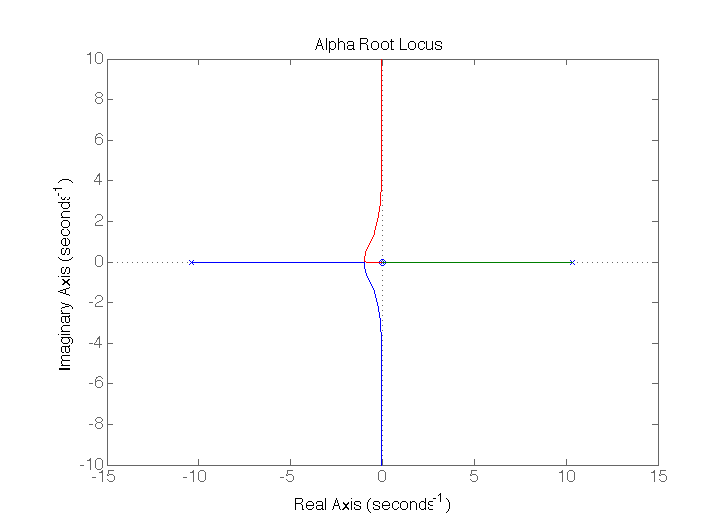
\includegraphics[width = 10cm]{alpha-1closedLoop.png}
\end{center}
\caption{180 Degree Root Locus of Transfer Function Relating $\alpha$ to input torque with a negative K}
\label{q8alphaInit}
\end{figure}

\begin{table}
\begin{center}
    \begin{tabular}{|c|c|c|c|c|}
        \hline
        Zeros & 0 & 0        & ~       & ~       \\ \hline
        Poles & 0 & -10.3814 & 10.3623 & -0.0177 \\
        \hline
    \end{tabular}
\caption{Poles and Zeros of equation \eqref{alphaTF2}}
\label{Alpharoots}
\end{center}
\end{table}

Substituting constants, we can get the open loop poles and zeros for the alpha transfer function, shown in table \ref{Alpharoots}. Because of the zero at the origin and the pole at the right half plane, all normal controllers such as lead, lead lag, PID, will all fail to bring that branch of the root locus out of the right half plane.  Our controller shown below in \eqref{alphaController} uses a pole at the origin to cancel the system zero and a pair of zeros to pull the root locus out of the right half plane.  We added a filtering pole to try and make the system more robust to noise.  The resulting system root locus is shown in figure  \ref{q8controlledAlpha}  The proportional gain term was chosen to make the dominant pair of poles critically damped.  

\begin{equation}
K_{2} = -3.7203\frac{(s - 3.75)(s - 7.85)}{s(s-50)} 
\label{alphaController}
\end{equation}

\begin{figure}
\begin{center}
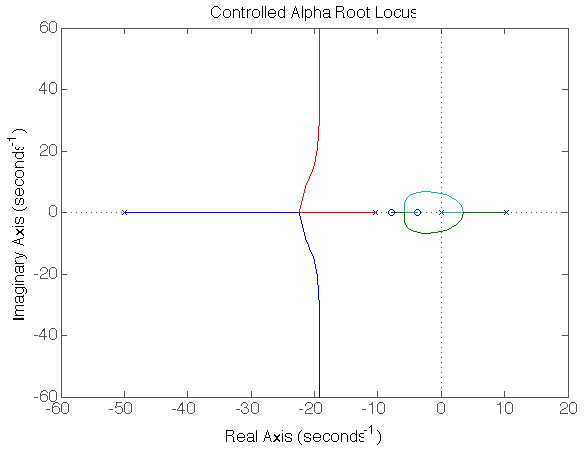
\includegraphics[width = 10cm]{controlledAlpha.png}
\end{center}
\caption{Root Locus for Alpha with Classical Controller}
\label{q8controlledAlpha}
\end{figure}

With the inner loop in place we now wish to control $\theta(s)$ which with just the inner loop is unstable and diverges.  First we must compute a new effective transfer function between the set point of the inner loop, $R_{\alpha}(s)$ and $\theta(s)$

\begin{equation}
\frac{\theta(s)}{R_{\alpha}(s)} = \frac{K_2(s)}{1 + K_2(s) G_2(s)} G_1(s)
\end{equation}

Numerically this transfer function is given by \eqref{numericaltfTwAC} with its 0 degree root locus shown in figure \ref{q8thetawAlphaControl}.

\begin{equation}
\frac{\theta(s)}{R_{\alpha}(s)} = \frac{-0.003596 \, s^4 - 0.04174\,  s^3 + 0.1503 \, s^2 + 2.974\, s + 7.549}{(1.078\e{-6}) s^6 + (5.394\e{-5}) s^5 + 0.002641 \, s^4 + 0.02615 \, s^3 + 0.08098 \, s^2}
\label{numericaltfTwAC}
\end{equation}

\begin{figure}
\begin{center}
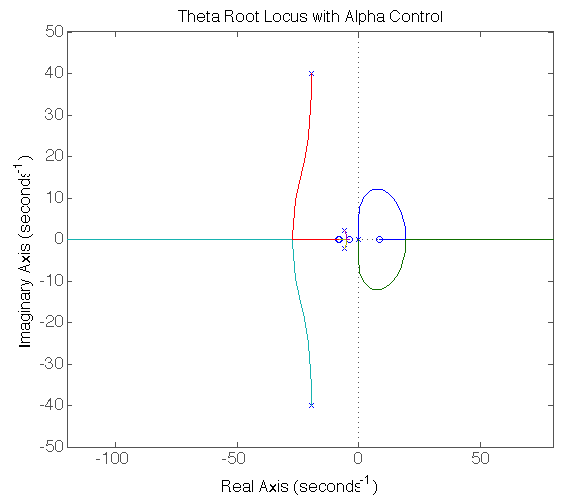
\includegraphics[width = 10cm]{thetaAlphaControl.png}
\end{center}
\caption{Transfer Function for Theta with Alpha Controlled}
\label{q8thetawAlphaControl}
\end{figure}

Normally we would like to design a controller that implements negative feedback, however in this case a positive feedback is appropriate and allows us to use a simple Lead Controller shown in \eqref{classicalK1} to obtain a stable root locus.

\begin{equation}
K_1(s) = 0.01784 \frac{s - 1}{s - 15}
\label{classicalK1}
\end{equation}

The resulting root locus for the controlled system is shown in figures \ref{q8controlledTheta} and \ref{q8controlledThetaDetail}.  It is worth noting that we are assured that alpha will remain stable regardless of what the outer loop does to the set point because all of its poles are in the left half plane, however this may not always be true due to the effects of saturation which could reduce our open loop gain and shift the poles into the right half plane. 

\begin{figure}
\begin{minipage}[b]{0.45\linewidth}
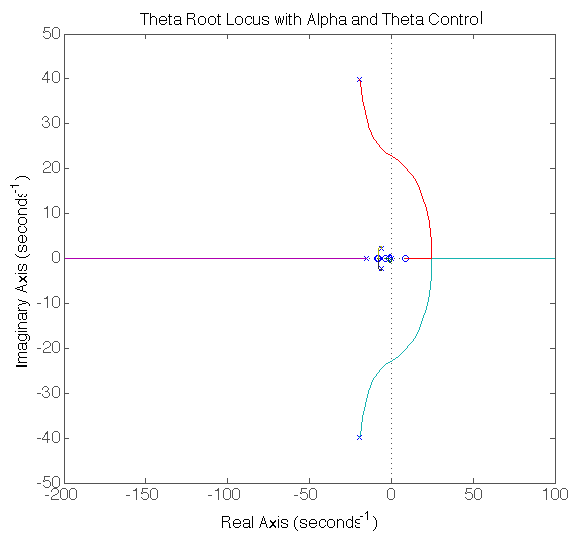
\includegraphics[width = 8cm]{controlledTheta.png}
\caption{Root Locus of Controlled $\theta$}
\label{q8controlledTheta}
\end{minipage}
\hspace{0.5cm}
\begin{minipage}[b]{0.45\linewidth}
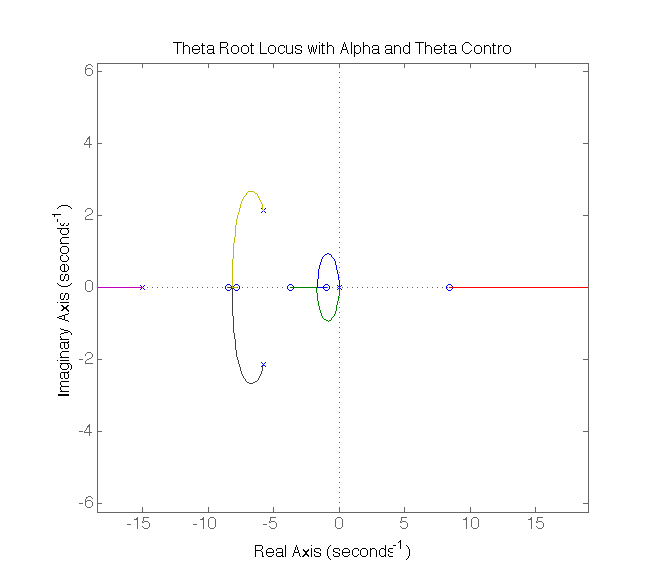
\includegraphics[width = 8cm]{controlledThetaDetail.png}
\caption{Detail of Root Locus to Left}
\label{q8controlledThetaDetail}
\end{minipage}
\end{figure}

With the classical controller constructed we first test it against the linear system model to confirm the design and it does prove to be stable, shown in \ref{ClassicalLinearModel}.  However we do notice that $\theta(t)$ has a very long settling time.  
\begin{figure}
\begin{center}
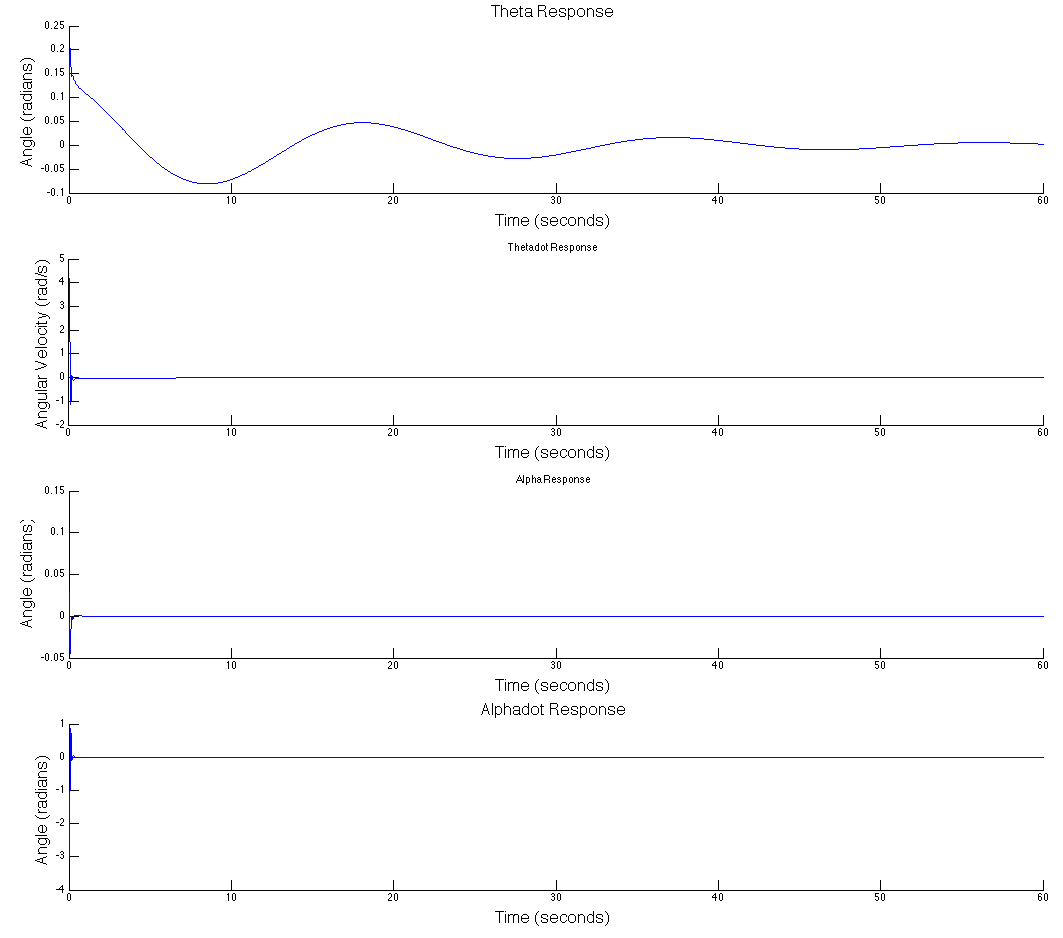
\includegraphics[width = 15cm]{classicalLinearModel.png}
\end{center}
\caption{The Classical Controller successfully stabilizes the linearized system, however $\theta$ has a long settling time}
\label{ClassicalLinearModel}
\end{figure}

\begin{figure}
\begin{center}
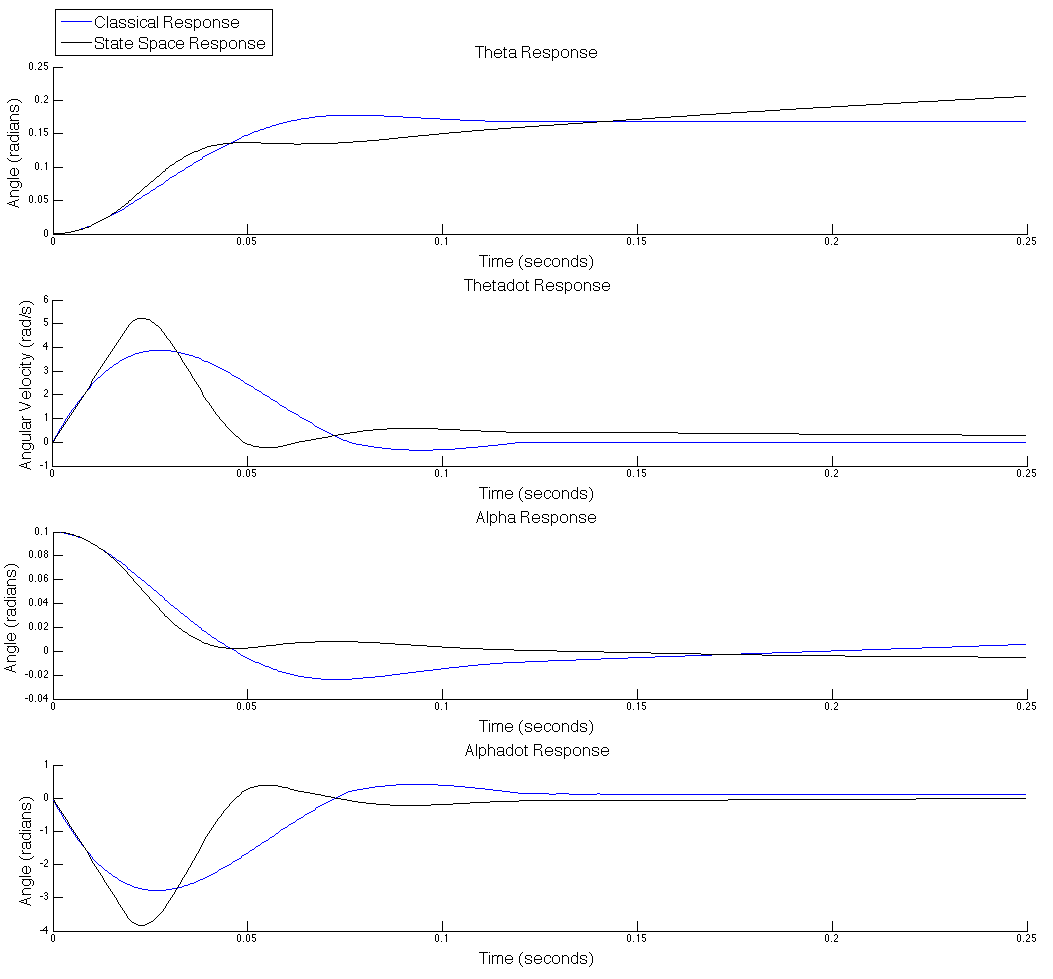
\includegraphics[width = 15cm]{transientNonLinear}
\end{center}
\caption{Comparison of the transient response of the non-linear model when controlled by the state-space controller and the classical controller.}
\label{q8classicalvsStateSpace}
\end{figure}

We next examine how using the non-linear model, which includes the effects of friction, impacts the performance of the controller.  Figure \ref{q8classicaltransientCompare} shows the limited effects of friction on the transient response.  There is actually a slight improvement with decreased overshoot.  However, when looking at the response over longer time scales, shown in figure \ref{ClassicalLimitCycle}, we see that the system exhibits a limit cycle likely caused by the friction.  

\begin{figure}
\begin{center}
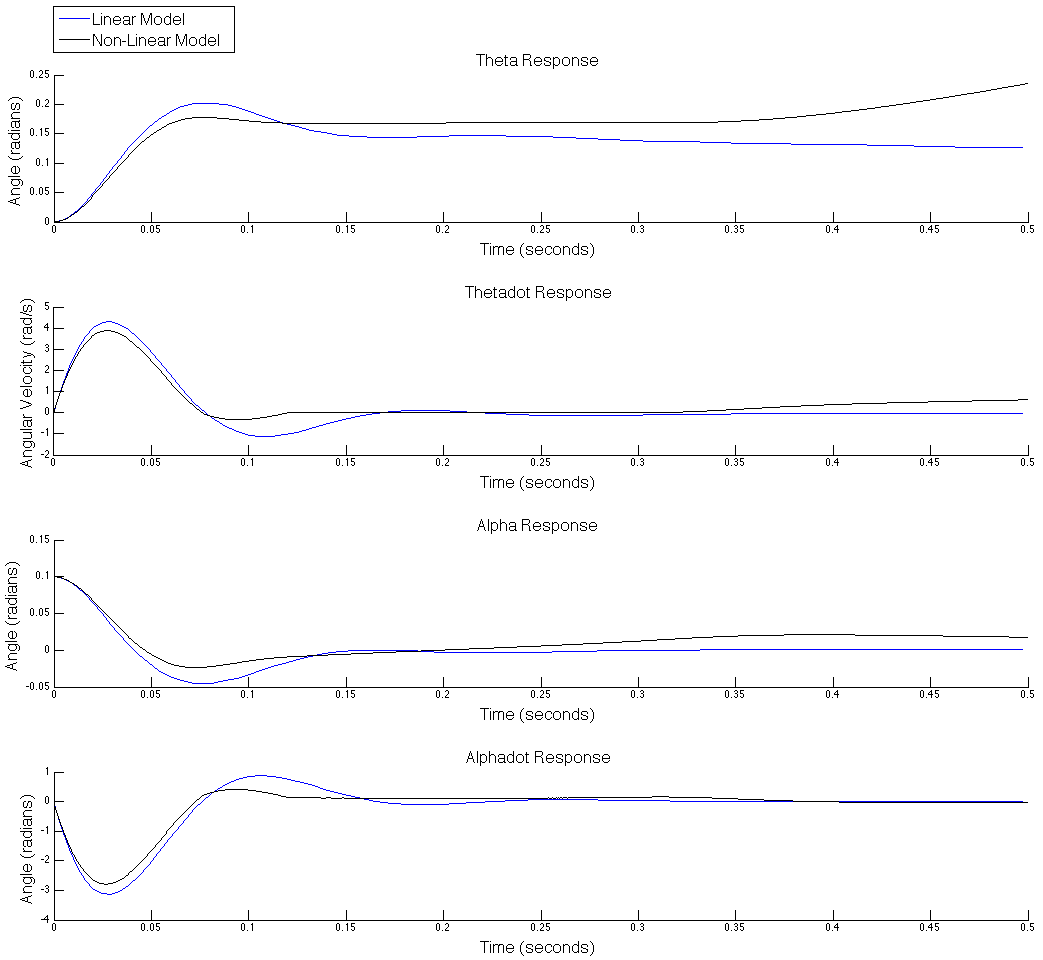
\includegraphics[width = 15cm]{classicaltransientLinearvsNonLinear.png}
\end{center}
\caption{The difference in the transient response of the classical controller applied to the linear and non-linear models}
\label{q8classicaltransientCompare}
\end{figure}

\begin{figure}
\begin{center}
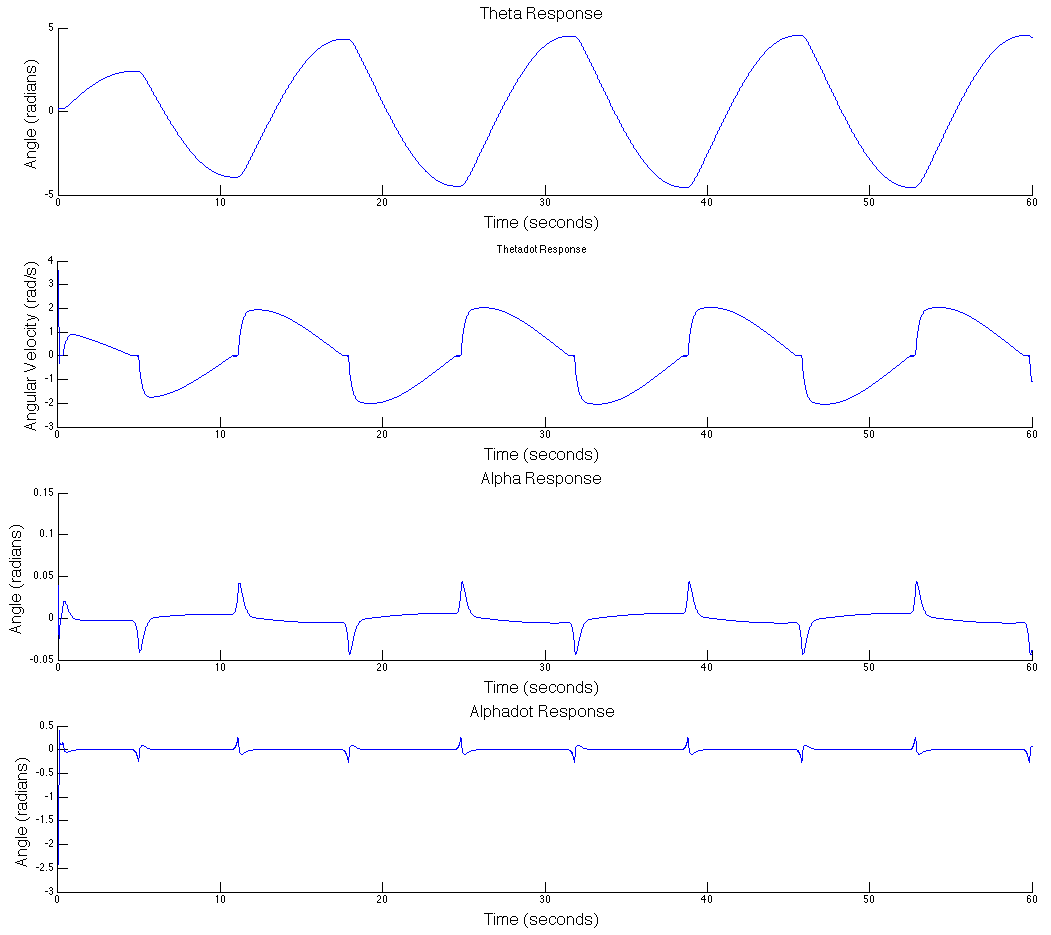
\includegraphics[width = 15cm]{ClassicalLimitCycle.png}
\end{center}
\caption{Limit cycle exerted by the classical controller when applied to the non-linear model for an initial $\alpha$ of 0.1 radians}
\label{ClassicalLimitCycle}
\end{figure}

Still in simulation, we also wish to compare the performance of the classical controller with the state space controller on the non-linear model.  We note as mentioned earlier, the state space controller exhibits a large steady state error for $\theta$ while the classical controller exhibits a large amplitude limit cycle.  Considering just the transient response we see that the state space controller responds slightly faster than the classical controller.  Simulation also claims that the classical controller is able to stabilize the pendulum starting from and initial angle, $\alpha_0$ up to $0.6125 radians$, while the state space controller has slightly worse performance being able stabilize initial $\alpha$ values up to $0.573 radians$.  However we do not expect to see performance this good in reality because the real controller is running at much lower loop rates than these simulated controllers which likely helps the simulations' stability.  Furthermore, there is no noise to corrupt our measurements and the models do not have to deal with un-modeled forces, specifically the cable which might limit our performance. 

Finally we implemented our classical controller in reality.  However the controller required some additional tuning of gains beyond the original design to successfully balance the pendulum, but this did result in a stable system.

$$K_{1 \, adjusted} = 0.2676\frac{s - 1}{s - 15} \hspace{1cm} K_{compensator \, adjusted} = 50 $$

Plugging these modified values back into our classical controller in Simulink resulted in a stable system and its response is plotted along side the response of the physical system in figure \ref{classicalSimulinkvsReal}.  We see a similarity between the $\theta$ plots.  Both experience limit cycles and our estimate of the amplitude and frequencies of this cycle do not seem to be very far off.  On the $\alpha$ plot we see a large difference in the initial transient response, with the real system oscillating rapidly before settling, while the simulated system overshoots once and quickly settles into its limit cycle.  All of our experiments so far have failed to produce smooth motion from the pendulum and this case is no different.  However we again note a similarity between the limit cycles in the two graphs.  We see that observed alpha shows very small peaks that correspond to $\dot{\theta}$ changing signs as our simulated system also shows. 

\begin{figure}
\begin{center}
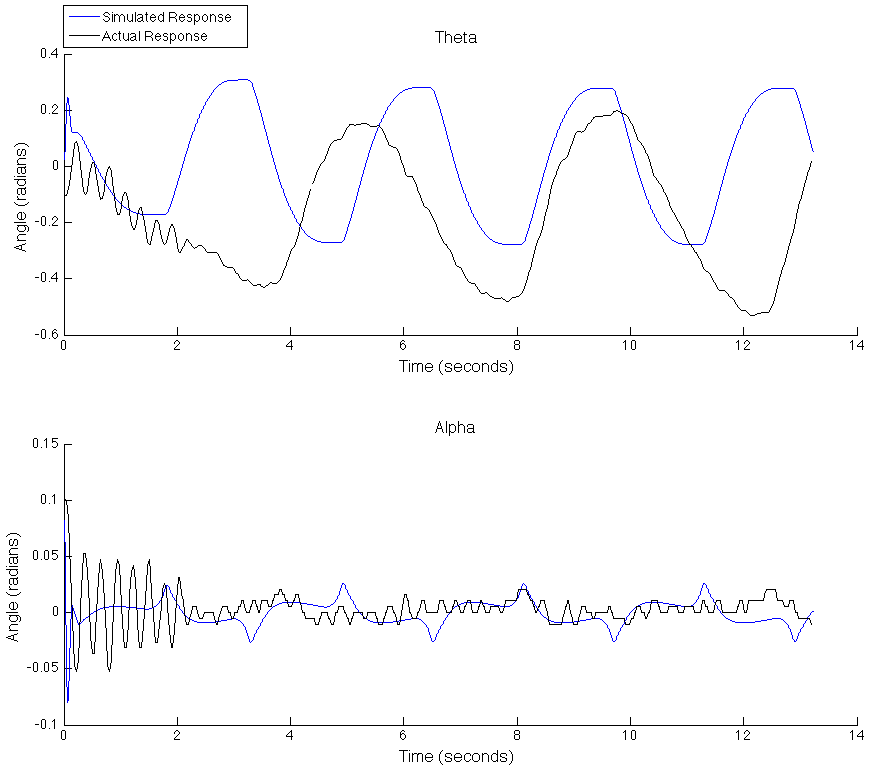
\includegraphics[width = 16cm]{modifiedrealvsSimulation.png}
\end{center}
\caption{Comparison of simulated non-linear system with modified gains against the real response}
\label{classicalSimulinkvsReal}
\end{figure}

Full state feedback control seems to be an easier system to design, simply construct a linear model of the system and run a function and we are given a set of values that work pretty well on the actual system.  The main disadvantage of this approach is that we lose all of the Laplace domain intuition learned from classical controls. However, in designing this classical controller we had already lost a great deal of that intuition and were left with playing with the root locus until a stable system appeared.  Despite these upsides, full state feedback has one major disadvantage compared to the classical controller.  All of the states must be observable for the method to work.  In this case we are forced to approximate the derivative using a lead controller which undoubtedly has negative consequences on performance and in other examples we may have no way of measuring the internal state of the system.  In this case classical controls methods are still applicable and may be able to produce a stable system. 



\clearpage
\section{Another Swing Up Controller}
When designing a new swing-up controller our goal was to use a very simple method that was still reliable. The controller we implemented shared some similarities with the method discussed in lecture, but simplified significantly. Rather than calculating the energy of the system or measuring the pendulum's position, our controller only looks at the direction of the pendulum and applies a constant voltage such that it switches sign every time the pendulum switches direction. Our goal was for the motor to apply high torque in one direction until the pendulum had stopped moving upwards, and then apply high torque in the opposite direction. With proper tuning of the voltage used, we believed we could meet the goal of only two swings before balancing. However, in practice we were not able to achieve this as our motor couldn't accelerate quickly enough to raise the pendulum sufficiently before its cords began twisting up too much. Therefore, we had to settle for a relatively low voltage command which required more swings. \\

Figure \ref{q9_1} shows the simplified balance controller implemented on the real system. We used a controller switch-over point of 0.3 radians (switching to our state-space balancer) and a command voltage of +- 3.0$V$ to get into balance mode in 19 swings (approximately 9.5 seconds). This was much worse than our prediction, which is shown in figure \ref{q9_2}. With our nonlinear simulink model we were able to reach balance mode in 4 swings (approximately 2.3 seconds) with a switch-over setting of 0.6 radians and a command voltage of +- 2.2$V$. Our controller on the real system requires a switch-over point much closer to the vertical position than the simulation does, which accounts for some of the difference in performance. Similarly, when we increased the command voltage to attempt to reduce the swings needed, the pendulum often overshot the vertical position and the balance controller was not able to catch it. Therefore, we decided to use a lower command input which takes more swings, but is much more reliable. Figures \ref{q9_3} and \ref{q9_4} show the simplified controllers as they were implemented in simulink and LabView, respectively. In all cases, the state-space balancer was used along with the simplified swing-up controller.\\

\begin{figure}[hbt]
\begin{center}
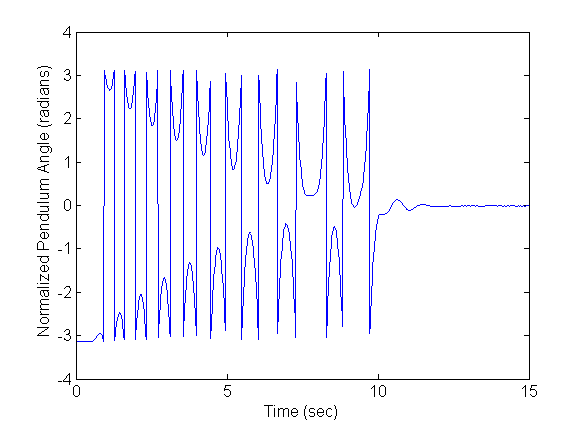
\includegraphics[width = 13cm]{Q9.png}
\end{center}
\caption{Simplified Swing-Up Controller on Real System}
\label{q9_1}
\end{figure}

\begin{figure}
\begin{center}
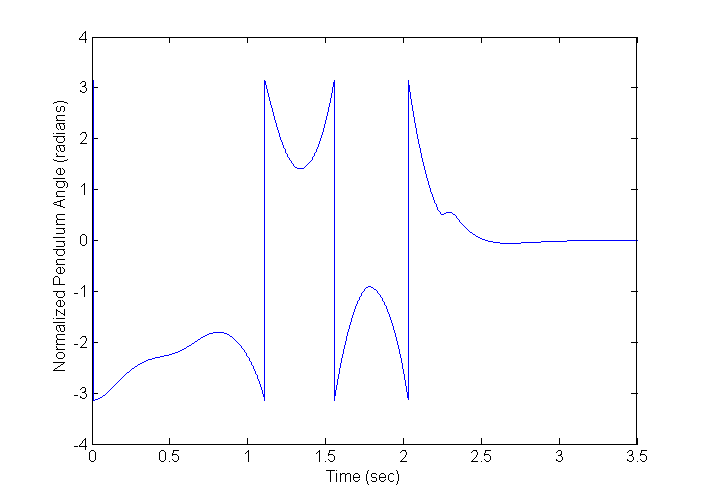
\includegraphics[width = 13cm]{Q9sim.png}
\end{center}
\caption{Simplified Swing-Up Controller with Nonlinear Simulink Model}
\label{q9_2}
\end{figure}

\begin{figure}
\begin{center}
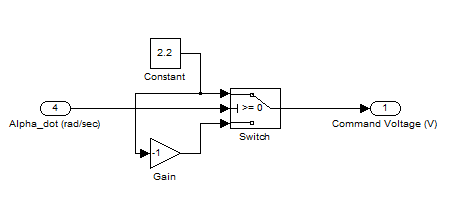
\includegraphics[width = 12cm]{Q9simulink.png}
\end{center}
\caption{Simplified Swing-Up Controller in Simulink Model}
\label{q9_3}
\end{figure}

\begin{figure}
\begin{center}
\includegraphics[width = 8cm]{Q9labview.png}
\end{center}
\caption{Simplified Swing-Up Controller in LabView}
\label{q9_4}
\end{figure}

\clearpage
\section{Parasitic Effects}
\begin{itemize}
\item Overview of Modeling Parasitic Effects
\begin{itemize}
\item Friction (see Fig.~\ref{fig:q10_1})\\
Frictional torque was incorporated into the equations of motion using the coulombic friction model presented in problem 1.  The frictional torques were identified experimentally.
\item Backlash/Deadband\\
Elastic behavior of the motor shaft and the coupling between the shaft and the horizontal arm could introduce backlash/deadband behavior.  The equations of motion were augmented to consider this effect. (Matlab function code).  
\item Quantization (see Fig.~\ref{fig:q10_3})\\
Two quantizer blocks were introduced to simulate the real behavior of optical encoders. According to the datasheets, the one used for measuring $\alpha$ has 1200 pulses per revolution (PPR), and the other one which measures $\theta$ has 2000 PPR with quadrature decoding.  
\item Discretization\\
Discretization was implemented by replacing all continuous Simulink blocks of the controller with discrete equivalents.  
\item Saturation (see Fig.~\ref{fig:q10_5})\\
The current limit of the servo amplifier was simulated through the addition of a $\pm$ 3V saturation block based on the datasheet to the command voltage.  Motor back-emf was simulated to limit maximum angular velocities using $K_b = K_t$.  
\item Noise (see Fig.~\ref{fig:q10_6})\\
The input and output disturbances were modeled separately. Noise sources, with a frequency of $60 Hz$ were added to the input to the motor driver and two the sensed $\theta$ and $\alpha$ values.  
\item Time Delay (see Fig.~\ref{fig:q10_7})\\
A time delay block was introduced between the "motor and driver model" and "Inverted Pendulum" blocks.    
\end{itemize}

\begin{figure}[h!]
\includegraphics[width=1\textwidth]{q10_1.png}
\caption{Modeling of Friction} \label{tex}
\label{fig:q10_1}
\end{figure}
\begin{figure}[h!]
\includegraphics[width=1\textwidth]{q10_3.png}
\caption{Modeling of Quantization} \label{tex}
\label{fig:q10_3}
\end{figure}
\begin{figure}[h!]
\includegraphics[width=1\textwidth]{q10_5.png}
\caption{Modeling of Saturation} \label{tex}
\label{fig:q10_5}
\end{figure}
\begin{figure}[h!]
\includegraphics[width=1\textwidth]{q10_6.png}
\caption{Modeling of Noise} \label{tex}
\label{fig:q10_6}
\end{figure}
\begin{figure}[h]
\includegraphics[width=1\textwidth]{q10_7.png}
\caption{Modeling of Time Delay} \label{tex}
\label{fig:q10_7}
\end{figure}


\item Friction (see Fig.~\ref{fig:q10_f1})\\
 Friction dissipates more energy and as a result, more swings are needed for the pendulum to reach the range of the balancing controller.  This increases the amount of time for the system to reach the balancing steady-state.
\begin{figure}[h]
\includegraphics[width=1\textwidth]{q10_f1.png}
\caption{Behavior of $\alpha$ with Friction On} \label{tex}
\label{fig:q10_f1}
\end{figure}

\item Backlash / Deadband (see Fig.~\ref{fig:q10_b1} and~\ref{fig:q10_b2})\\
Introducing backlash causes the system to take more time to reach the steady state. Furthermore, the magnitude of $\dot{\theta}$ seems to be smaller when swinging up but it oscillates within a small range during the balancing stage.
\begin{figure}[h]
\includegraphics[width=1\textwidth]{q10_b1.png}
\caption{Behavior of $\alpha$ with Friction On} \label{tex}
\label{fig:q10_b1}
\end{figure}
\begin{figure}[h]
\includegraphics[width=1\textwidth]{q10_b2.png}
\caption{Behavior of $\dot{\theta}$ with Friction On} \label{tex}
\label{fig:q10_b2}
\end{figure}

\item Quantization (see Fig.~\ref{fig:q10_q1},~\ref{fig:q10_q2} and~\ref{fig:q10_q3})\\
In the real system, both optical encoders introduce quantization to the angle measurements. The simulation results show that during steady state, oscillations occur in $\alpha$ and $\theta$.  Unlike the original model which outputs very nearly zero torque, these oscillations in the angle measurements cause oscillations in motor torque, within the range of $0.2 Nm$ to compensate for the perceived error.   
\begin{figure}[h]
\includegraphics[width=1\textwidth]{q10_q1.png}
\caption{Behavior of $\dot{\alpha}$ with Quantization} \label{tex}
\label{fig:q10_q1}
\end{figure}
\begin{figure}[h]
\includegraphics[width=1\textwidth]{q10_q2.png}
\caption{Behavior of $\dot{\theta}$ with Quantization} \label{tex}
\label{fig:q10_q2}
\end{figure}
\begin{figure}[h]
\includegraphics[width=1\textwidth]{q10_q3.png}
\caption{Behavior of Motor Toque with Quantization} \label{tex}
\label{fig:q10_q3}
\end{figure}

\item Discretization (see Fig.~\ref{fig:q10_d1})\\
The simulation results suggest that the system with discrete-time control performs better during the swing-up stage, reaching steady state sooner. However, if we increase the time step to a certain degree (Ts=0.005), the system becomes unstable, which means the discretization affects the system stability.
\begin{figure}[h]
\includegraphics[width=1\textwidth]{q10_d1.png}
\caption{Behavior of $\alpha$ with Discretization} \label{tex}
\label{fig:q10_d1}
\end{figure}

\item Saturation (see Fig.~\ref{fig:q10_s1} and~\ref{fig:q10_s2})\\
As can be seen in Fig.~\ref{fig:q10_s1} and~\ref{fig:q10_s2}, more time is required for the first swing when the saturation is considered. It suggests that previously large torque was available to provide sufficient energy for the pendulum system to swing at the beginning, but now more time is needed to add the same amount of energy with the limited torque.      

\begin{figure}[h]
\includegraphics[width=1\textwidth]{q10_s1.png}
\caption{Behavior of $\alpha$ with Saturation} \label{tex}
\label{fig:q10_s1}
\end{figure}
\begin{figure}[h]
\includegraphics[width=1\textwidth]{q10_s2.png}
\caption{Behavior of Motor Torque with Saturation} \label{tex}
\label{fig:q10_s2}
\end{figure}

\item Noise (see Fig.~\ref{fig:q10_n1}~\ref{fig:q10_n2} and~\ref{fig:q10_n3})\\
Both input and output disturbances have similar undesired influence on the system performance. Despite the tiny difference when the swing-up controller is working, during the balancing stage, oscillations occur in the $\alpha$ and $\theta$. The range of oscillations depends on the magnitudes of noise. Noise added to sensor measurements has the greatest impact resulting in motor torques applied to the system during steady state.  

\begin{figure}[h]
\includegraphics[width=1\textwidth]{q10_n1.png}
\caption{Behavior of $\dot{\alpha}$ with Noise} \label{tex}
\label{fig:q10_n1}
\end{figure}
\begin{figure}[h]
\includegraphics[width=1\textwidth]{q10_n2.png}
\caption{Behavior of $\dot{\theta}$ with Noise} \label{tex}
\label{fig:q10_n2}
\end{figure}
\begin{figure}[h]
\includegraphics[width=1\textwidth]{q10_n3.png}
\caption{Behavior of Motor Torque with Noise} \label{tex}
\label{fig:q10_n3}
\end{figure}

\item Time Delay (see Fig.~\ref{fig:q10_t1},~\ref{fig:q10_t2} and~\ref{fig:q10_t3})\\
In the physical model, the dynamic response of the servo-amplifier, encoders, and NI-DAQ are assumed instantaneous. In order to simulate the real behavior, a small time delay was introduced to our simulink model. For the swing-up stage, time delay has a small effect which  simply causes the same amount of time shift. However, during the balancing stage, time delay has strong negative impact on the balancing control. $\alpha$ vibrates significantly as the time delay is increased; thus, the motor behaves aggressively and large torque is required during the transient response.     This behavior in steady state resembles the oscillations seen in the real system and we may conclude that time delay is contributing to the poor system behavior.

\begin{figure}[h]
\includegraphics[width=1\textwidth]{q10_t1.png}
\caption{Behavior of $\alpha$ with Time Delay} \label{tex}
\label{fig:q10_t1}
\end{figure}
\begin{figure}[h]
\includegraphics[width=1\textwidth]{q10_t2.png}
\caption{Behavior of $\theta$ with Time Delay} \label{tex}
\label{fig:q10_t2}
\end{figure}
\begin{figure}[h]
\includegraphics[width=1\textwidth]{q10_t3.png}
\caption{Behavior of Motor Torque with Time Delay} \label{tex}
\label{fig:q10_t3}
\end{figure}
\end{itemize}

\clearpage
\section*{Appendix.}

\subsection*{Equation of Motion from Lagrange Method}
\verbatiminput{eqMotionLagrange.m}

\subsection*{Linearized Equation of Motion about $\alpha = 0$}
\verbatiminput{eqMotionLinear.m}

\subsection*{Linearized Equation of Motion about $\alpha = \pi$}
\verbatiminput{eqMotionLinearDown.m}

\subsection*{Envelop Extraction}
\verbatiminput{extractEnvelop.m}

\subsection*{Variable Initialization for Linear Simulink model}
\verbatiminput{LinearPrelim.m}

\subsection*{Angle Normalization}
\verbatiminput{mod2pi.m}

\subsection*{Pendulum Equation of Motion}
\verbatiminput{pendulumEQMotion.m}

\subsection*{Prototype for Pendulum Parameter Regression}
\verbatiminput{pendulumEstimation.m}

\subsection*{Helper Function}
\verbatiminput{polyCoadd.m}

\subsection*{Motor supply voltage saturation modeling}
\verbatiminput{saturation.m}

\subsection*{Variable Initialization for State Space Controller}
\verbatiminput{StateSpacePrelimv2.m}

\subsection*{System Energy Computation}
\verbatiminput{totalEnergy.m}

\end{document}